% Nota: El corrector ortográfico que utilizo solo tiene soporte para inglés y español.
% Es por eso que lo deshabilito en las zonas donde hay mucho texto en un idioma distinto a estos dos.

% spell-checker: disable

%%%%%%%%%%%%%%%%%%%%%%%%%%%%%%%%%%%%%%%%%%%%%%%%%%%%%%%%%%%%%%%%%%%%%%%%%%%%%%%
%                       CARREGA DE LA CLASSE DE DOCUMENT                      %
%                                                                             %
% Les opcions admissibles son:                                                %
%      12pt / 11pt            (cos dels tipus de lletra; no feu servir 10pt)  %
%                                                                             %
% catalan/spanish/english     (llengua principal del treball)                 %
%                                                                             % 
% french/italian/german...    (si necessiteu fer servir alguna altra llengua) %
%                                                                             %
% listoffigures               (El document inclou un Index de figures)        %
% listoftables                (El document inclou un Index de taules)         %
% listofquadres               (El document inclou un Index de quadres)        %
% listofalgorithms            (El document inclou un Index d'algorismes)      %
%                                                                             %
%%%%%%%%%%%%%%%%%%%%%%%%%%%%%%%%%%%%%%%%%%%%%%%%%%%%%%%%%%%%%%%%%%%%%%%%%%%%%%%

\documentclass[11pt,spanish,listoffigures,listoftables,table,hyphens,dvipsnames]{tfgetsinf}

%%%%%%%%%%%%%%%%%%%%%%%%%%%%%%%%%%%%%%%%%%%%%%%%%%%%%%%%%%%%%%%%%%%%%%%%%%%%%%%
%                     CODIFICACIO DEL FITXER FONT                             %
%                                                                             %
%    windows fa servir normalment 'ansinew'                                   %
%    amb linux es possible que siga 'latin1' o 'latin9'                       %
%    Pero el mes recomanable es fer servir utf8 (unicode 8)                   %
%                                          (si el vostre editor ho permet)    % 
%%%%%%%%%%%%%%%%%%%%%%%%%%%%%%%%%%%%%%%%%%%%%%%%%%%%%%%%%%%%%%%%%%%%%%%%%%%%%%%

\usepackage[utf8]{inputenc} 

%%%%%%%%%%%%%%%%%%%%%%%%%%%%%%%%%%%%%%%%%%%%%%%%%%%%%%%%%%%%%%%%%%%%%%%%%%%%%%%
%                        ALTRES PAQUETS I DEFINICIONS                         %
%                                                                             %
% Carregueu aci els paquets que necessiteu i declareu les comandes i entorns  %
%                                          (aquesta seccio pot ser buida)     %
%%%%%%%%%%%%%%%%%%%%%%%%%%%%%%%%%%%%%%%%%%%%%%%%%%%%%%%%%%%%%%%%%%%%%%%%%%%%%%%

\usepackage{tablefootnote}
\usepackage{alltt}

\usepackage{pgfplots}
\pgfplotsset{compat=1.16}

\newcommand{\fe}[1]{\foreign{english}{#1}}

%%%%%%%%%%%%%%%%%%%%%%%%%%%%%%%%%%%%%%%%%%%%%%%%%%%%
% https://tex.stackexchange.com/questions/147836/emphasize-color-contents-between-two-delimiters-in-listings-but-not-the-delim

\def\beginlstdelim#1#2#3%
{%
   \def\endlstdelim{#2\egroup}%
   #1\bgroup\color{#3}\aftergroup\endlstdelim%
}

%%%%%%%%%%%%%%%%%%%%%%%%%%%%%%%%%%%%%%%%%%%%%%%%%%

\definecolor{purple}{HTML}{BE5AC7} % 'HTML' means hex code
\definecolor{stringgreen}{HTML}{91B46E}
\definecolor{lightblue}{HTML}{6DB0CC}
\definecolor{grey}{HTML}{676E95}
\definecolor{firestoregreen}{HTML}{39A676}

\lstdefinelanguage{none}{
   identifierstyle=
}

\lstdefinestyle{verbatim}{
   language=none,
   basicstyle=\small\ttfamily,
   breaklines=true,
   numbers=none,
   frame=none
}

\lstdefinelanguage{TypeScript}{
   keywords={public, protected, private, class, interface, typeof, new, true, false, try, catch, throw, function, switch, var, let, const, if, in, while, do, else, case, break, async},
   keywordstyle=\color{purple}\bfseries,
   morekeywords=[2]{import, export, as, from, return, null, await},
   keywordstyle=[2]\color{lightblue},
   morekeywords=[3]{Promise, RequestInterceptor, ResponseInterceptor, RequestHandler, string, any, boolean, Response, HandlerInput},
   keywordstyle=[3]\color{orange},
   moredelim=**[is][\beginlstdelim{\color{purple}\textbf{new}}{\color{black}(}{orange}]{new}{(},
   moredelim=**[is][\beginlstdelim{\color{purple}\textbf{class}}{\color{black}\{}{orange}]{class}{\{},
   moredelim=**[is][\beginlstdelim{\color{purple}\textbf{interface}}{\color{black}\{}{orange}]{interface}{\{},
   identifierstyle=\color{black},
   sensitive=true,
   comment=[l]{//},
   morecomment=[s]{/*}{*/},
   commentstyle=\color{grey},
   stringstyle=\color{stringgreen},
   morestring=[b]',
   morestring=[b]",
   % String interpolation
   morestring=**[d]{`},
   moredelim=**[is][\beginlstdelim{\color{stringgreen}\$\{}{\color{stringgreen}\}}{black}]{\$\{}{\}}
}

\lstdefinestyle{TypeScript-no-dots}{
   language=TypeScript
}

\lstdefinestyle{TypeScript-dots}{
   language=TypeScript,
   moredelim=**[is][\beginlstdelim{.}{(}{blue}]{.}{(},
}

\lstdefinelanguage{Firestore}{
   keywords={service, match, allow, if},
   morekeywords=[2]{read, write, request, auth, uid},
   morekeywords=[3]{null, true, false},
   keywordstyle=\color{blue},
   keywordstyle=[2]\color{firestoregreen},
   keywordstyle=[3]\color{orange},
   stringstyle=\color{orange},
   morestring=[b]'
}

\lstdefinelanguage{Dart}{
   keywords={public, protected, private, new, void, switch, var, const, if, in, while, do, else, case, break, static, final, @override},
   keywordstyle=\color{purple}\bfseries,
   morekeywords=[2]{class, extends, return, null, await, true, false, try, catch, async, get},
   keywordstyle=[2]\color{lightblue},
   morekeywords=[3]{Future, String, bool, Intl, MaterialApp, GlobalMaterialLocalizations, GlobalWidgetsLocalizations, GlobalCupertinoLocalizations, AppLocalizationsDelegate, AppLocalizations, Locale, Widget, BuildContext},
   keywordstyle=[3]\color{orange},
   moredelim=**[is][\beginlstdelim{\color{purple}\textbf{new}}{\color{black}(}{orange}]{new}{(},
   moredelim=**[is][\beginlstdelim{\color{purple}\textbf{class}}{\color{black}\{}{orange}]{class}{\{},
   moredelim=**[is][\beginlstdelim{\color{purple}\textbf{interface}}{\color{black}\{}{orange}]{interface}{\{},
   identifierstyle=\color{black},
   sensitive=true,
   comment=[l]{//},
   morecomment=[s]{/*}{*/},
   commentstyle=\color{grey},
   stringstyle=\color{stringgreen},
   morestring=[b]',
   morestring=[b]"
}

\lstdefinelanguage{YAML}{
   identifierstyle=\color{olive},
   moredelim=**[il][\beginlstdelim{\color{black}:\ \ }{\color{MidnightBlue}}{MidnightBlue}]{:\ },
   moredelim=**[il][\beginlstdelim{\color{black}-\ \ }{\color{MidnightBlue}}{MidnightBlue}]{-\ },
   morestring=[b]",
   stringstyle=\color{Maroon},
   comment=[l]{\#},
   commentstyle=\color{OliveGreen}
}

\lstset{
   language=TypeScript,
   %columns=flexible,
   keepspaces=true,
   style=TypeScript-dots,
   literate=%
      {Á}{{\'A}}1
      {É}{{\'E}}1
      {Í}{{\'I}}1
      {Ó}{{\'O}}1
      {Ú}{{\'U}}1
      {á}{{\'a}}1
      {é}{{\'e}}1
      {í}{{\'i}}1
      {ó}{{\'o}}1
      {ú}{{\'u}}1
}

\def\arraystretch{1.5}

%%%%%%%%%%%%%%%%%%%%%%%%%%%%%%%%%%%%%%%%%%%%%%%%%%%%%%%%%%%%%%%%%%%%%%%%%%%%%%%
%                        DADES DEL TREBALL                                    %
%                                                                             %
% titol, alumne, tutor i curs academic                                        %
%%%%%%%%%%%%%%%%%%%%%%%%%%%%%%%%%%%%%%%%%%%%%%%%%%%%%%%%%%%%%%%%%%%%%%%%%%%%%%%

% spell-checker: enable

\title{Al Loro: \\
         Lector de \fe{feeds RSS} para asistente de voz}
\author{Alejandro Gómez Noé}
\tutor{Vicente Pelechano Ferragud}
\curs{2020-2021}

% spell-checker: disable

%%%%%%%%%%%%%%%%%%%%%%%%%%%%%%%%%%%%%%%%%%%%%%%%%%%%%%%%%%%%%%%%%%%%%%%%%%%%%%%
%                     PARAULES CLAU/PALABRAS CLAVE/KEY WORDS                  %
%                                                                             %
% Independentment de la llengua del treball, s'hi han d'incloure              %
% les paraules clau i el resum en els tres idiomes                            %
%%%%%%%%%%%%%%%%%%%%%%%%%%%%%%%%%%%%%%%%%%%%%%%%%%%%%%%%%%%%%%%%%%%%%%%%%%%%%%%

% spell-checker: enable

\keywords
         % spell-checker: disable-next-line
         {Alexa, assistent de veu, Alexa skills, RSS, Atom, notícies, blogs, podcasts} % Paraules clau 
         {Alexa, asistente de voz, Alexa skills, RSS, Atom, noticias, blogs, podcasts} % Palabras clave
         {Alexa, voice assistant, Alexa skills, RSS, Atom, news, blogs, podcasts}      % Key words

%%%%%%%%%%%%%%%%%%%%%%%%%%%%%%%%%%%%%%%%%%%%%%%%%%%%%%%%%%%%%%%%%%%%%%%%%%%%%%%
%                              INICIO DEL DOCUMENTO                           %
%%%%%%%%%%%%%%%%%%%%%%%%%%%%%%%%%%%%%%%%%%%%%%%%%%%%%%%%%%%%%%%%%%%%%%%%%%%%%%%

\begin{document}

%%%%%%%%%%%%%%%%%%%%%%%%%%%%%%%%%%%%%%%%%%%%%%%%%%%%%%%%%%%%%%%%%%%%%%%%%%%%%%%
%           RESÚMENES DEL TFG EN VALENCIANO, CASTELLANO E INGLÉS              %
%%%%%%%%%%%%%%%%%%%%%%%%%%%%%%%%%%%%%%%%%%%%%%%%%%%%%%%%%%%%%%%%%%%%%%%%%%%%%%%

% spell-checker: disable

\begin{abstract}
   Últimament, els assistents de veu estan tornant-se molt populars (\emph{Amazon Alexa}, \emph{Assistent de Google}, etc.), i ofereixen als desenvolupadors ferramentes per a crear les seues pròpies aplicacions compatibles amb aquests sistemes. Concretament, en Alexa es diuen \emph{``skills''}, i és possible insta{\lgem}ar-les solament amb la veu. Un tipus de \textit{skill} són els butlletins de notícies, els quals funcionen a través de \emph{feeds RSS/Atom}. El principal problema amb elles és que, per a què sigan compatibles amb Alexa, aquestes \textit{feeds} han de tindre un format molt precís, i és molt inusual que ho complisquen. Per aquest motiu, l'objectiu d' aquest treball és el d'implementar una \textit{skill} on pugues afegir les teues \textit{feeds} favorites, i escoltar notícies, blogs, podcasts... a través d'aquesta \textit{skill}. A l'hora d'afegir una \textit{feed}, podràs configurar aspectes com ara el seu nom, el seu idioma (amb soport per a espanyol i anglès), el màxim de notícies que et deuria llegir, o quant text deuria llegirte d'una vegada. La configuració es realitzarà a través d'una app, on podràs gestionar les teues \textit{feeds}.
\end{abstract}

% spell-checker: enable

\begin{abstract}[spanish]
   Últimamente, los asistentes de voz se están volviendo muy populares (\emph{Amazon Alexa}, \emph{Asistente de Google}, etc.), y ofrecen a los desarrolladores herramientas para crear sus propias aplicaciones compatibles con estos sistemas. Concretamente, en Alexa se llaman \emph{``skills''}, y es posible instalarlas sólo con la voz. Un tipo de \textit{skill} son los boletines de noticias, los cuales funcionan a través de \emph{feeds RSS/Atom}. El principal problema con ellas es que, para que sean compatibles con Alexa, estas \textit{feeds} deben tener un formato muy preciso, y es muy inusual que lo cumplan. Por este motivo, el objetivo de este trabajo es el de implementar una \textit{skill} donde puedas añadir tus \textit{feeds} favoritas, y escuchar noticias, blogs, podcasts... a través de dicha \textit{skill}. A la hora de añadir una \textit{feed}, podrás configurar aspectos como su nombre, su idioma (con soporte para español e inglés), el máximo de noticias que te debería leer, o cuánto texto debería leerte de una vez. La configuración se realizará a través de una app, donde podrás gestionar tus \textit{feeds}.
\end{abstract}

\begin{abstract}[english]
   Lately, voice assistants are becoming really popular (\emph{Amazon Alexa}, \emph{Google Assistant}, etc.), and they offer developers tools to make their own applications compatible with these systems. More specifically, in Alexa they are called \emph{``skills''}, and it is possible to install them just by voice. One kind of \textit{skill} are news briefers, which work through \emph{RSS/Atom feeds}. The main issue with them is that, for them to be compatible with Alexa, these \textit{feeds} must have a very precise format, and it is very unlikely to find any that complies with it. For this reason, this project's objective is to implement a \textit{skill} where you can add your favorite \textit{feeds}, and listen to news articles, blogs, podcasts... through said \textit{skill}. When adding a \textit{feed}, you will be able to configure aspects such as its name, language (with support for english and spanish), the maximum number of news articles it should read to you, or how much text it should read at once. This configuration will be done through an app, where you will be able to manage your \textit{feeds}.
\end{abstract}

%%%%%%%%%%%%%%%%%%%%%%%%%%%%%%%%%%%%%%%%%%%%%%%%%%%%%%%%%%%%%%%%%%%%%%%%%%%%%%%
%                              CONTENIDO DEL TRABAJO                          %
%%%%%%%%%%%%%%%%%%%%%%%%%%%%%%%%%%%%%%%%%%%%%%%%%%%%%%%%%%%%%%%%%%%%%%%%%%%%%%%

\mainmatter

%%%%%%%%%%%%%%%%%%%%%%%%%%%%%%%%%%%%%%%%%%%%%%%%%%%%%%%%%%%%%%%%%%%%%%%%%%%%%%%
%                                  INTRODUCCIÓN                               %
%%%%%%%%%%%%%%%%%%%%%%%%%%%%%%%%%%%%%%%%%%%%%%%%%%%%%%%%%%%%%%%%%%%%%%%%%%%%%%%

\chapter{Introducción}

Durante los últimos años, Internet ha ido formando cada vez más parte de nuestras vidas, especialmente a la hora de obtener información (noticias, entretenimiento, etc.). Medios más tradicionales como la televisión o la radio han ido perdiendo relevancia frente a las redes sociales, y estos se han visto obligados a adaptarse a las nuevas tecnologías.

Por otro lado, los dispositivos móviles (como teléfonos o tabletas inteligentes) se han convertido en nuestro principal medio de consumo de contenido a través de Internet, debido a su facilidad de uso y portabilidad. Esto podemos observarlo gracias a la popularidad de las \fe{apps}, y por tanto, del desarrollo móvil.

Pero, desde hace bastante poco, y gracias a la mejora exponencial de los sistemas de procesamiento del lenguaje natural, un nuevo competidor ha llegado al mercado: los asistentes de voz, que permiten hacer todo tipo de cosas sin mover un dedo. Empresas del calibre de Amazon y Google están invirtiendo muchos recursos en este campo con sus respectivas soluciones: Amazon Alexa y el Asistente de Google.

Ambas están disponibles para dispositivos móviles, pero también existen unos dispositivos diseñados específicamente para estos asistentes de voz: Amazon Echo y Google Nest.

Para el presente trabajo, nos centraremos en los servicios de Amazon: el asistente Alexa y los dispositivos Echo (podemos observar uno de sus modelos en la figura~\ref{figura:echo-dot}).

\begin{figure}[ht]
   \centering
   \includegraphics[width=0.23\textwidth]{echo-dot.png}
   \includegraphics[width=0.20\textwidth]{echo-dot-2.png}
      \caption{Dispositivo Amazon Echo Dot (4ª Generación, con reloj)}
   \label{figura:echo-dot}
\end{figure}

Gracias a estos asistentes, podemos hacer cosas como: crear alarmas, recordatorios; preguntar acerca del tiempo, el tráfico, o las noticias del día... entre otras.

Además, los asistentes de voz tienen una especial integración con la domótica: bombillas, enchufes, termostatos... son algunos ejemplos de dispositivos en los que algunas empresas han incluido soporte para poder ser controlados desde Alexa.

Pero la cosa no acaba ahí: también permite a los desarrolladores crear sus propias aplicaciones compatibles con Alexa, llamadas \emph{skills}.

\section{Motivación}

Hace unos meses adquirí un dispositivo Echo Dot, y empecé a experimentar con sus diferentes funcionalidades. Como estudiante de Ingeniería de Software, me llamó especialmente la atención el desarrollo de skills y las posibilidades que ello permite.

Tras investigar un poco al respecto, descubrí que las skills funcionan mediante el servicio \emph{AWS Lambda}. En su página principal en español\footnote{\url{https://aws.amazon.com/es/lambda/}} lo definen como
<<un servicio informático sin servidor que le permite ejecutar código sin aprovisionar ni administrar servidores>>. Este tipo de servicios son conocidos como \fe{serverless}, y se han vuelto bastante populares en los últimos años.

Los servicios en la nube son muy demandados, útiles e interesantes; y considero una buena inversión de cara al futuro poder aprender más acerca de ellos. Además, este proyecto sirve como introducción en un campo novedoso y con (probablemente) mucho futuro por delante como es el de los asistentes de voz.

Por otro lado, el desarrollo de la skill me ha servido para aprender sobre un lenguaje de programación del que he oído hablar mucho últimamente: \emph{TypeScript}\footnote{\url{https://www.typescriptlang.org}}. Se trata de una extensión del lenguaje \emph{JavaScript}, al que le añade un sistema de tipos. Esto, junto a otras características del lenguaje, mejora sustancialmente la experiencia de desarrollo, y ha llevado a muchas grandes empresas a migrar su código \emph{JavaScript} hacia \emph{TypeScript} (además de haber propiciado una mayor adopción por parte del público general).

\section{Objetivos}

El principal objetivo de este trabajo es \textbf{documentar el proceso de desarrollo de una skill}, poniendo énfasis en el uso de técnicas y herramientas ya establecidas en el desarrollo de otro tipo de aplicaciones más comunes.

Uno de los mayores impedimentos a la hora de introducirse en el entorno de Alexa es el trabajo previo de investigación que requiere. Por ello, se busca \textbf{proporcionar una guía que sirva de referencia para implementar skills}, y que se centre en los siguientes aspectos:

\begin{itemize}
   \item Sus similitudes con el desarrollo \emph{backend}, mediante el uso de los servicios de \emph{AWS} y el modelo \emph{serverless}.
   \item Las opciones a la hora de integrar o complementar una skill con otro tipo de aplicaciones y servicios (\emph{apps}, bases de datos, etc.)
   \item El funcionamiento (a nivel del desarrollador de skills) de una interfaz guiada por voz, y cómo diseñar un modelo conversacional.
\end{itemize}

Uno de los aspectos más útiles en una guía o documentación es la existencia de \textbf{ejemplos prácticos} extraídos de un \textbf{producto software funcional}, que permitan al desarrollador obtener una visión más completa del propósito de cada pequeña funcionalidad que se trata en la guía.

Para ello, se plantea el objetivo de \textbf{implementar una skill} que \textbf{solucione un problema real} o \textbf{mejore un modelo existente}. En el contexto de este trabajo se tratará de <<\emph{Al Loro}>>, una skill de noticias que proporcionará una mejor integración con las feeds \emph{RSS} con respecto de la funcionalidad existente en el propio sistema de Alexa.

\section{Estructura}

Los próximos capítulos seguirán la siguiente estructura:

\begin{itemize}
   \item \textbf{\nameref{capitulo:estado-arte}}

      Se hará una comparativa de los principales asistentes de voz disponibles en el mercado, comentando sus fortalezas y debilidades, y se justificará la elección de asistente para este trabajo.
   \item \textbf{\nameref{capitulo:analisis-problema}}

      Se comentará la dificultad para desarrolladores que la documentación en este trabajo del desarrollo de ``Al Loro'' puede ayudar a aliviar, y el problema con la lectura de noticias en Alexa del que nació la skill como posible solución.
   \item \textbf{\nameref{capitulo:diseno-solucion}}
      
      Se repasará la arquitectura del sistema que conforma ``Al Loro'', profundizando en los diferentes subsistemas y el proceso de decisión de las tecnologías utilizadas en los mismos.
      
      También se analizará con mayor detalle el diseño de la skill en sí misma: la estructura del proyecto, las diferentes partes por las que está formado (interfaz, lógica, persistencia) y cómo se relacionan estos conceptos en el desarrollo de skills.
   \item \textbf{\nameref{capitulo:desarrollo-solucion}}
   
      Se revisará el proceso de desarrollo del sistema, analizando las diferentes librerías y herramientas utilizadas, así como el proceso de aprendizaje y los contratiempos que surgieron durante la implementación.
   \item \textbf{\nameref{capitulo:implantacion}}
   
      Se explicará el funcionamiento de la fase de certificación y publicación de una skill en Alexa. Además, se mostrará un proceso similar en el contexto de la publicación de la app complementaria en la \emph{Google Play Store} (la tienda de aplicaciones para Android).
   \item \textbf{\nameref{capitulo:pruebas}}

      Se introducirán los principales conceptos relacionados con la fase de pruebas del proyecto (las pruebas unitarias y el análisis estático), junto con las herramientas utilizadas para ponerlos en práctica.
   \item \textbf{\nameref{capitulo:conclusiones}}
   
      Se resumirá el contenido de los capítulos anteriores, relacionándolo con los objetivos iniciales y con asignaturas cursadas en el grado.

\end{itemize}

Para comprender mejor aquellas palabras o expresiones que sean técnicas o específicas de la temática de este trabajo y se repitan a lo largo del mismo, existe un \hyperref[glosario]{\textbf{glosario}} al final del documento.

%%%%%%%%%%%%%%%%%%%%%%%%%%%%%%%%%%%%%%%%%%%%%%%%%%%%%%%%%%%%%%%%%%%%%%%%%%%%%%%
%                      CAPÍTULOS (tantos como haga falta)                     %
%%%%%%%%%%%%%%%%%%%%%%%%%%%%%%%%%%%%%%%%%%%%%%%%%%%%%%%%%%%%%%%%%%%%%%%%%%%%%%%

%%%%%%%%%%%%%%
% CAPÍTULO 2 %
%%%%%%%%%%%%%%

\chapter{Estado del arte} % Contexto Tecnológico
\label{capitulo:estado-arte}

\section{Asistentes de voz}

Existen tres principales asistentes de voz en el mercado: Asistente de Google\footnote{\url{https://assistant.google.com/intl/es_es/}}, Amazon Alexa\footnote{\url{https://developer.amazon.com/es-ES/alexa}}, y Siri\footnote{\url{https://www.apple.com/es/siri/}} (de la compañía Apple). La tabla \ref{tabla:voice-assistant-comparison} muestra una comparativa entre ellos.

\begin{table}[ht]
   \centering
   \begin{tabular}{@{}|>{\raggedright\small}p{0.22\linewidth}|>{\raggedright\small}p{0.22\linewidth}|>{\raggedright\small}p{0.22\linewidth}|>{\raggedright\arraybackslash\small}p{0.22\linewidth}| @{}}
      \hline
      & \normalsize Google & \normalsize \textbf{Alexa} & \normalsize Siri \\
      \hline
      Kits de desarrollo & \emph{Actions}~\cite{google-assistant-docs} & \emph{Skills}~\cite{alexa-skills-docs} & \emph{SiriKit}~\cite{siri-docs} \\
      \hline
      Lenguajes soportados & JavaScript (Node.js) & JavaScript (Node.js), Python & Swift, Objective-C \\
      \hline
      Plataformas & Android, Google Home & Amazon Echo, Fire TV, Android e iOS\tablefootnote{Es necesario instalar la app de Amazon Alexa para poder utilizar dicho asistente en Android e iOS.} & iOS, HomePod \\
      \hline
      Mayor enfoque & Búsqueda por Internet & \emph{Skills}, domótica, entretenimiento & Productividad \\
      \hline 
   \end{tabular}
   \caption{Comparativa de los asistentes de voz más populares}
   \label{tabla:voice-assistant-comparison}
\end{table}

\subsection{Asistente de Google}

Se trata de uno de los asistentes de voz más populares en el mercado, puesto que se encuentra instalado por defecto en el sistema operativo con mayor presencia en dispositivos móviles: Android.

Su principal atractivo es su sistema de \textbf{búsqueda por Internet}. Google cuenta con el motor de búsqueda más utilizado, y lo aprovecha al máximo integrándolo en el asistente.

Su kit de desarrollo, \textbf{\emph{Google Actions}}, busca facilitar el aprendizaje y mejorar la experiencia de desarrolladores \textbf{principiantes} y entusiastas. Integrando en su consola una herramienta de modelado basada en \textbf{diagramas} (figura \ref{figura:google-actions-console}), el proceso de desarrollo obtiene un enfoque más \textbf{visual}, lo cual ayuda a introducirse en el flujo de trabajo habitual de este tipo de programas: uno más centrado en el \textbf{modelo conversacional} y el \textbf{árbol de decisiones}.

Aun así, no deja de lado a los desarrolladores más avanzados, ya que provee de una funcionalidad llamada <<\textbf{\emph{webhooks}}>> con la que poder integrar una API personalizada, ya sea mediante un \emph{endpoint} HTTPS o haciendo uso del servicio <<\emph{Cloud Functions}>> que ofrece la plataforma Firebase (un servicio de Google).

\begin{figure}[ht]
   \centering
   \includegraphics[width=\textwidth]{google-actions-console.jpg}
   \caption{Herramienta de modelado basada en diagramas - \emph{Google Actions Console}}
   \label{figura:google-actions-console}
\end{figure}

\subsection{Amazon Alexa}

Pese a tener el menor uso en dispositivos móviles de los tres, Alexa es un gran contendiente en el marco de los dispositivos \fe{Smart Home}, gracias a su familia de productos Amazon Echo.

Su sistema de búsqueda por Internet es el peor de los tres con diferencia\footnote{En un estudio~\cite{voice-search-study} de la empresa \emph{SEMrush} realizado en el año 2020, el porcentaje de preguntas que quedaron sin respuesta usando Alexa fue de un 23\%, mientras que en el resto de asistentes era menor del 10\%.}, pero trata de compensarlo con su enfoque en la \textbf{integración con otras plataformas}. Con una gran inversión en su sistema de \textbf{\emph{skills}}, Alexa busca que desarrolladores de todo tipo implementen aplicaciones para poder hacer uso de sus sistemas a través de este asistente de voz.

Entre las categorías de skills más destacadas se encuentran:

\begin{itemize}
   \item \textbf{Entretenimiento}: Juegos y curiosidades, cuentos para niños, meditación, recetas de cocina\dots
   \item \textbf{Hogar digital} (\fe{Smart Home}): Skills de domótica asociadas a dispositivos como bombillas inteligentes, cámaras de vigilancia, o termostatos.
   \item \textbf{Multimedia}: Dan acceso a servicios de música o vídeo, como cadenas de radio o \fe{podcasts}.
   \item \textbf{Noticias}: Servicios de noticias tanto de televisión, radio, periódicos, revistas, e incluso independientes (por ejemplo, a través de YouTube).
\end{itemize}

En cuanto a la plataforma de \emph{skills}, su curva de \textbf{aprendizaje} es un \textbf{término medio} entre las otras dos. Como ofrece una integración con los lenguajes \textbf{\emph{JavaScript}} y \textbf{\emph{Python}} en forma de librerías especializadas, el \textbf{desarrollador web} es el más beneficiado, con una mayor facilidad de adaptación debido al uso extensivo de tecnologías web conocidas en el kit de desarrollo.

\subsection{Siri}

Este asistente dispone de un público más selecto, pues sólo se encuentra disponible en productos de la marca Apple (como el \emph{iPhone} o el \emph{iPad}), los cuales tienen una base de usuarios más reducida. Sin embargo, estos son más proclives a utilizar Siri, llevando a algunas encuestas a mostrar alrededor de un 45\% de cuota relativa de mercado en \fe{smartphones} de los Estados Unidos~\cite{voice-assistant-market-share}.

Respecto a su conjunto de funcionalidades, no parece haber una que destaque especialmente sobre el resto en cuanto a su promoción. Aun así, muchas comparten una misma temática: la \textbf{productividad}. Su publicidad está enfocada en la comodidad y rapidez que aporta utilizar Siri para realizar tareas cotidianas. Un ejemplo de ello son los \textbf{atajos}: un sistema para, según la página principal de Siri,  <<agilizar las tareas que haces más a menudo>> mediante <<una serie de funciones rápidas muy útiles>> que encadenan una sucesión de acciones.

El kit de desarrollo de Siri (\textbf{\emph{SiriKit}}) está fuertemente acoplado al ecosistema de \emph{iOS} y su desarrollo de apps -- de hecho, toda interacción con los sistemas de Siri debe ser hecha desde una app desarrollada para el sistema operativo móvil de Apple\footnote{También existen las <<\emph{app extensions}>> (\url{https://developer.apple.com/documentation/sirikit/intent_handling_infrastructure/structuring_your_code_to_support_app_extensions}), intermediarios que actúan en nombre de la app; pero suelen requerir de un alto grado de integración con la propia app de iOS.}.

Por este motivo, esta plataforma de desarrollo es la \textbf{menos abierta} a nuevos desarrolladores; ya que, como mínimo, se requiere de:

\begin{itemize}
   \item Un conocimiento general del lenguaje de programación (\emph{Swift}), el cual es utilizado casi exclusivamente en productos de Apple.
   \item Un ordenador de la familia de Mac, para tener acceso al editor de código \emph{XCode} y sus herramientas, sin las cuales no se pueden compilar apps\footnote{Algunos frameworks multiplataforma como \emph{Flutter} permiten crear apps para Android e iOS, pero sin \emph{XCode} no se puede generar el producto final en iOS.} para iOS.
\end{itemize}

\section{Propuesta}

Este trabajo se centrará en el desarrollo de skills para \emph{Amazon Alexa}. Como dispone de un mayor nivel de inversión y popularidad que los kits de desarrollo de la competencia, es más probable que tenga éxito de cara al futuro; lo cual hace que sea un tema de estudio interesante.

Al tratarse de un campo novedoso, es muy probable que muchos desarrolladores con otras especialidades (desarrollo web o móvil, por ejemplo) empiecen a interesarse por Alexa y traten de adaptar sus sistemas existentes a este nuevo medio. Por este motivo, en los próximos capítulos se va a aportar una nueva visión desde esta perspectiva.

%%%%%%%%%%%%%%
% CAPÍTULO 3 %
%%%%%%%%%%%%%%

\chapter{Análisis del problema}
\label{capitulo:analisis-problema}

\section{Lectura de noticias}

Entre los modelos de skill pre-construidos que Alexa proporciona (figura \ref{figura:skill-models}), se encuentra el modelo de noticias~\cite{flash-briefing-skills-doc}, el cual no requiere ningún conocimiento de programación, sino un simple enlace a una \hyperref[glosario:feed]{\emph{feed}} con el estándar \emph{RSS} o con formato \emph{JSON} y una estructura concreta. Técnicamente, este modelo permite añadir contenido de blogs, páginas de noticias, etc. para que Alexa lo lea. Pero también tiene varios problemas que presentamos en las siguientes subsecciones:

\subsection{Intención de uso del modelo de noticias}

Este sistema no está pensado para que un usuario añada el contenido de sus webs favoritas, sino para que los dueños de estas webs creen sus propias skills con este contenido para que luego sus usuarios las puedan instalar y consumirlo.

De hecho, no se puede publicar una skill de este tipo salvo que quien lo haga sea dueño del contenido que incluye, o disponga de permiso para distribuirlo de esta forma~\cite{flash-briefing-skill-policy-guidelines}.

En principio, un usuario podría crear estas skills y mantenerlas para uso personal (pues sólo estarían disponibles al público tras un riguroso proceso de certificación~\cite{flash-briefing-skill-certification-process}), pero sería poco conveniente, pues tendría que: o crear una skill para cada uno de los servicios de noticias que utilice, lo cual sería un proceso tedioso y poco razonable; o tener una sola skill para todos sus servicios, caso en el que tendría poco control sobre cuál de ellos desea escuchar en cada momento. Además, si no es un desarrollador, es poco probable que sepa de esto (ni quiera hacerlo).

\subsection{Formato esperado de una feed}

El modelo requiere una feed \textit{RSS} (o \textit{JSON}). En términos muy simples, se trata de una lista con los diferentes artículos, ya sean noticias, entradas de un blog, etc. Estos artículos tienen varios campos. Los más importantes serían el título y la descripción.
   
Muchos sitios incluyen el título de la noticia en el campo ``título'', y el subtítulo en el campo ``descripción''. Si lees una noticia, el subtítulo no es más que una extensión del título, dependiente de este.

Pues bien, el modelo de noticias de Alexa únicamente lee al usuario el campo ``descripción'', y no el campo ``título''~\cite{flash-briefing-skill-feed-format-details}. Esto lleva a que, cuando te lee una noticia, esta queda inconclusa, puesto que te lee el subtítulo, pero no el título.
   
En el caso de los blogs no es tan grave, ya que en el campo ``descripción'' suelen incluir el contenido de la publicación (en algunos casos completo, en otros sólo un segmento). 

Pero, aun así, el título es lo más importante; puesto que te resume en pocas palabras su contenido, y te sirve para decidir rápidamente si te interesa o no. Es más, en algunos casos, no puedes comprender el contenido de la publicación sin leer su título --especialmente si el contenido está resumido--.

Esto lleva a situaciones en las que se le lee al usuario un contenido que resulta no interesarle, pero no lo sabe hasta que lo ha leído entero.

Por otro lado, uno de los requisitos para una feed es que su contenido se encuentre en texto plano y no contenga caracteres especiales~\cite{flash-briefing-skill-text-content-requirements}. Muchos sitios no lo cumplen, y por tanto no pueden ser utilizados para crear una skill de este tipo.

\section{Modelado Conceptual}

Los casos de uso de la skill (figura \ref{figura:diagrama-casos-uso}) son relativamente sencillos, pues la función principal es leer feeds, y para ello no hacen falta muchos más comandos. Obtener una lista de las feeds disponibles para saber qué feeds se pueden leer y recibir ayuda acerca de los comandos disponibles y cómo llamarlos son las otras dos funcionalidades básicas de la skill.

Sin embargo, existe una función un tanto más compleja en el contexto de una aplicación guiada por voz: gestionar las feeds. Añadir, editar o eliminar feeds no sólo es un proceso tedioso por voz, sino que no es viable porque requiere indicar enlaces web. Por tanto, se utiliza una app para proveer estos servicios. Mediante un sistema de autenticación basado en un código de seis dígitos, la app puede gestionar la lista de feeds de la que la skill hace uso.

\begin{figure}[ht]
   \centering
   \includegraphics[width=\textwidth]{diagrama-casos-de-uso.png}
   \caption{Diagrama de casos de uso}
   \label{figura:diagrama-casos-uso}
\end{figure}

Para la función de leer una feed, es importante mostrar un diagrama de flujo (figura \ref{figura:diagrama-flujo}) para ver con más detalle el proceso en base a la experiencia del usuario.

En otras circunstancias, el proceso podría ser más sencillo, pero debido a algunas características y limitaciones de Alexa, se han tomado varias decisiones:

\begin{itemize}
   \item Al comenzar el proceso de lectura de una feed, el usuario puede haber proporcionado previamente su nombre al ejecutar el comando, pero también puede no haberlo hecho. Por suerte, Alexa se encarga de esta situación\footnote{Se trata de una función que hay que activar y configurar desde la consola de Alexa, pero no hace falta gestionarlo por código.}, pidiendo al usuario el nombre de la feed si no la tiene.
   \item Debido a una limitación en el número de caracteres permitidos en una respuesta, el contenido de feeds más largas debe ser dividido en secciones. Cada vez que acaba de leer una sección, Alexa pregunta al usuario si quiere que siga leyendo (siempre y cuando quede contenido por leer).
\end{itemize}

\begin{figure}[ht]
   \centering
   \includegraphics[width=\textwidth]{diagrama-flujo.png}
   \caption{Diagrama de flujo para el caso de uso ``Leer una feed''}
   \label{figura:diagrama-flujo}
\end{figure}

Entrando en un apartado más técnico, el siguiente modelo es un diagrama de clases de aquellos objetos relacionados con las feeds (figura \ref{figura:diagrama-clases}).

La característica más llamativa de este modelo es la falta de métodos entre las clases. Esto se debe a una limitación en la forma en la que Alexa almacena los objetos entre peticiones de una misma sesión. Cada vez que una petición termina de ser manejada, aquellos objetos que quieran ser persistidos deben convertirse a texto para ser incluidos en la respuesta; y así podrán ser recuperados en la siguiente petición. Por desgracia, durante este proceso los métodos de los objetos se pierden y dejan de ser accesibles. Es por eso que todas las funciones se definen de forma separada, y las clases sólo contienen los datos estrictamente necesarios.

Por este mismo motivo, las clases del diagrama están realmente definidas como <<\emph{interfaces}>>: estructuras que indican al sistema de tipos de TypeScript cómo debería estar formado un objeto de JavaScript (el cual es dinámico y puede tener la estructura que quiera). Las interfaces son eliminadas en el proceso de compilación, y sólo sirven para mejorar la experiencia de desarrollo y detectar posibles \fe{bugs}.

Otras particularidades del diagrama de clases son:

\begin{itemize}
   \item La existencia de una clase <<\emph{Feed}>> que deriva de otra llamada <<\emph{FeedData}>> y sólo contiene un atributo de más, el nombre.
   
   La idea detrás de esto es que en la base de datos, el nombre está almacenado en dos atributos según el idioma del dispositivo: inglés y español.
   
   Esto se puede configurar desde la app, y permite al usuario cambiar el idioma de su dispositivo cuando le plazca y seguir teniendo acceso a su lista de feeds con nombres adecuados.

   Al iniciarse la skill, se detecta el idioma actual del dispositivo y se obtiene el atributo adecuado. Primero se indica al sistema de tipos que no existe aún un atributo <<nombre>> usando \emph{FeedData}, y una vez añadido se redefine su tipo\footnote{<<Redefinir el tipo>> sólo se refiere a cambiar la interfaz que define la estructura del objeto. El tipo <<real>> sigue siendo el de <<objeto>> a secas, así que a nivel de ejecución no tiene ningún efecto.} como \emph{Feed}.

   \item La relación entre las clases <<\emph{FeedData}>> y <<\emph{FeedItems}>>. De nuevo, se debe a la limitación que no permite tener la función <<\emph{getItems(FeedData)}>> como método de la clase <<\emph{FeedData}>>.
   
   En este caso, <<\emph{FeedData}>> representa el conjunto de datos que el usuario ha indicado en la app (y, por tanto, se encuentra en la base de datos); mientras que <<\emph{FeedItems}>> contiene el resultado de obtener las noticias de la feed, tras haber sido procesado y ordenado en un formato más cómodo para el código encargado de leer las noticias.
\end{itemize}

Por otro lado, este diagrama incluye dos funcionalidades que, aunque no son esenciales, pueden resultar bastante útiles:

\begin{itemize}
   \item Soporte para podcasts: Algunas feeds pueden formar parte de un podcast, e incluir un enlace a un capítulo en cada elemento. En esos casos, la skill pregunta al usuario si quiere escucharlo tras haber leído todo el contenido de texto. En caso afirmativo, hace uso del sistema de reproducción de audio de Alexa para ponerlo en marcha.
   \item Filtros para feeds: Algunos sitios de noticias abarcan una gran variedad de temas entre su contenido, y al usuario no tienen por qué interesarle todos. Por eso, desde la app se pueden indicar una serie de textos y/o categorías para que sólo aparezcan aquellos elementos que los contengan. También se puede indicar si tienen que coincidir todos, o si cualquiera de ellos sirve para darlo por bueno.
\end{itemize}

\begin{figure}[ht]
   \centering
   \includegraphics[width=\textwidth]{diagrama-clases-feed.png}
   \caption{Diagrama de clases (Feed)}
   \label{figura:diagrama-clases}
\end{figure}

\section{Solución propuesta}

Visto el funcionamiento del actual modelo de noticias, es interesante plantear una posible alternativa: una skill a través de la cual el usuario pueda añadir sus propias feeds y escuchar su contenido, sin depender de que sus dueños sepan de la existencia de Alexa y decidan invertir tiempo en crear su propia skill de noticias.

Del mismo modo, se puede aprovechar su proceso de desarrollo para profundizar en los diferentes aspectos de la creación de skills en Alexa, como:

\begin{itemize}
   \item Sus similitudes con el desarrollo \emph{backend}, mediante el uso de los servicios de \emph{AWS} y el modelo \emph{serverless}.
   \item Las opciones a la hora de integrar o complementar una skill con otro tipo de aplicaciones y servicios (\emph{apps}, bases de datos, etc.)
   \item El funcionamiento (a nivel del desarrollador de skills) de una interfaz guiada por voz, y cómo diseñar un modelo conversacional.
\end{itemize}

%%%%%%%%%%%%%%
% CAPÍTULO 4 %
%%%%%%%%%%%%%%

\chapter{Diseño de la solución}
\label{capitulo:diseno-solucion}

\section{Arquitectura del Sistema}

El sistema está dividido en tres grandes subsistemas, mostrados en la figura \ref{figura:diagrama-bloques}:

\begin{itemize}
   \item \textbf{Amazon}: Se trata del subsistema principal, puesto que contiene al propio servicio de Alexa y la skill. Además, engloba una serie de servicios de una cuenta de AWS independiente, los cuales se encuentran integrados con la skill para añadirle la funcionalidad necesaria para comunicarse con la app.
   \item \textbf{Firebase}\footnote{\url{https://firebase.google.com/}}: Este servicio de base de datos de Google se encarga de persistir las feeds. Además, proporciona un servicio de autenticación para poder gestionarlas a través de la app. 
   \item \textbf{App}: Desarrollada mediante el \fe{framework} de Google \emph{Flutter}\footnote{\url{https://flutter.dev/}}, permite al usuario gestionar sus feeds fácilmente. 
\end{itemize}

\begin{figure}[ht]
   \centering
   \includegraphics[width=\textwidth]{diagrama-bloques.png}
      \caption[Diagrama de bloques]{Diagrama de bloques representando la arquitectura del sistema\\
      \footnotesize (los servicios en gris están disponibles pero no son utilizados)}
   \label{figura:diagrama-bloques}
\end{figure}

\subsection{Sistema de gestión de feeds}

\subsubsection{Otras arquitecturas contempladas}

Inicialmente se buscaron opciones tratando de que toda la funcionalidad de cara al usuario pudiera existir dentro de la skill (es decir, que fuera posible interaccionar con ella mediante la voz), pero se acabó considerando que esto no era posible en el caso de la introducción de los enlaces a las diferentes feeds. Esto se debe a que el texto de un enlace no tiene por qué ser pronunciable (o fácilmente comprensible por Alexa), lo cual podría provocar frustración al usuario.

Tras verse frustrado el plan ideal, se barajaron alternativas en las que puedas introducir estos datos de manera escrita. En primer lugar, se investigó si existía alguna tecnología así entre los servicios de Alexa, para que sirviera de apoyo a la skill sin tratarse de una aplicación aparte.

Esto llevó al descubrimiento del \emph{APL} (\fe{Alexa Presentation Language}): un lenguaje a través del cual, según su página dedicada en la documentación de Alexa~\cite{apl-doc}, puedes crear una serie de <<documentos>> que aportan <<experiencias visuales que acompañan a la skill>>, con las cuales los usuarios pueden también interactuar.

Sin embargo, su uso se acabó tachando de inviable, debido a que está limitado a aquellos dispositivos con pantalla propia (<<el Echo Show, la Fire TV, algunas tabletas Fire, y otros dispositivos>>, según la documentación), y no parece estar disponible a través de la app Alexa\footnote{Se utiliza la expresión ``parece'' porque esto no se menciona en la documentación. Sin embargo, en el foro de Alexa existen comentarios donde se indica que no está disponible.}. Es por ello que aquella funcionalidad que aporte no debería ser esencial; es decir, todo aquello que se pueda hacer gracias a APL, debería poder hacerse también por voz. 

\subsubsection{Decisión final y sus ventajas}

Tras esta investigación, se llegó a la conclusión de que la skill por sí sola no resultaría suficiente para conseguir toda la funcionalidad deseada, y sería necesaria una aplicación complementaria para la gestión de las feeds. Dicha aplicación podría ser web, de escritorio o móvil.

La aplicación de escritorio fue la primera en descartarse, pues no aporta nada que no se pueda hacer a través de una web, y estaría disponible en un menor número de dispositivos.

Entre la aplicación web y móvil, surgió la siguiente coyuntura:

\begin{itemize}
   \item Por un lado, la aplicación web sería más versátil, al estar disponible tanto para ordenadores como dispositivos móviles.
   
   \item Pero por otro lado, una aplicación móvil sería menos costosa en cuanto a horas de trabajo, al disponer de mayor experiencia en su desarrollo. Además, el uso de dispositivos móviles está muy extendido, por lo que la falta de versatilidad no sería tan grave.
\end{itemize}

Finalmente, se optó por desarrollar una aplicación móvil (o app, para abreviar).

\subsection{Integración entre la skill y la app}

Tras decidir que la existencia de una app para gestionar las feeds es necesaria, el siguiente paso es averiguar cómo integrar ambos servicios para que funcionen conjuntamente.

\subsubsection{Base de datos}

En primer lugar, se requiere un sistema de base de datos común al que puedan acceder ambas aplicaciones. Aquí se valoraron dos opciones:

\begin{itemize}
   \item Amazon dispone del servicio \emph{DynamoDB}, accesible por parte de la skill desde su creación. Sin embargo, la integración de éste con la app resulta bastante más compleja, y su curva de aprendizaje es relativamente alta.
   \item En cambio, el servicio de Google \textbf{\emph{Cloud Firestore}} (de la familia de productos \emph{Firebase}) tiene una integración más sencilla con la app, y acceder a él a través de la skill no tiene mucha complicación.
\end{itemize}

\subsubsection{Autenticación}
\label{seccion:auth}

En segundo lugar, es necesario un sistema de autenticación para la app. Aquel que se utilice debe ser compatible tanto con la base de datos como con la skill, ya que esta última es la que proporciona identificadores de usuario. Además, el proceso de inicio de sesión debe ser fácil y cómodo para el usuario. Y sería preferible que no tenga que proporcionar credenciales de ninguna cuenta que pueda provocar reticencia al usuario, como Google o Amazon\footnote{Este argumento surgió a partir de un comentario presente en la página de una skill similar a esta, donde era tildada de ``estafa'' por requerir un inicio de sesión en Google para utilizar una página web complementaria.}.

Como resultado, se ideó un sistema de autenticación mediante un \textbf{código} de 6 dígitos. El procedimiento es el que sigue:

\begin{enumerate}
   \item Desde la skill, el usuario indica que desea iniciar sesión. Alexa genera y dicta el código que podrá utilizar para ello. Internamente, dicho código se ha asociado a su usuario mediante un identificador y se ha almacenado en una base de datos (\textit{DynamoDB}).
   \item El usuario accede a la app, e introduce el código que Alexa le ha dictado. Por su parte, la app realiza una petición a una \emph{API}, que a su vez se dedicará a validar que el código se encuentra en la base de datos que la skill utiliza para guardar los códigos. En caso afirmativo, se generará un \textit{token} que la app recibirá como respuesta, y con el que podrá iniciar sesión a través del servicio de autenticación correspondiente.
\end{enumerate}

Respecto a los servicios disponibles para las bases de datos anteriormente mencionadas, las opciones son:

\begin{itemize}
   \item Por parte de Amazon, se encuentra \emph{Cognito}\footnote{\url{https://aws.amazon.com/es/cognito/}}. Este servicio forma parte de \emph{AWS}. Posee una amplia variedad de funcionalidades, pero al mismo tiempo resulta más complejo.
   \item Entre los productos de Google, \textbf{\emph{Firebase Authentication}}\footnote{\url{https://firebase.google.com/products/auth?hl=es}} (o \emph{Auth} para abreviar) sería la solución. Es más sencillo de configurar que el anterior, y posee una opción de autenticación personalizada, lo cual permite la creación de un sistema por código.
\end{itemize}

Las soluciones empleadas fueron las de Google: la familia de productos \emph{Firebase}.

Un aspecto a comentar es que, para generar un token, es necesario un identificador de usuario. Aunque, como se ha mencionado antes, la skill proporciona uno, este es demasiado largo para el servicio de autenticación utilizado. Por otro lado, la base de datos genera un identificador más corto por cada documento creado con los datos de un usuario. Es por ello que se utiliza este último para generar los \emph{tokens}. Debido a esto, la \emph{API} que valida los códigos ha de realizar una llamada extra a la base de datos para ``traducir'' el identificador (es decir, obtener la versión corta a partir de la larga).

\section{Diseño Detallado}

\subsection{Estructura de directorios}

\begin{table}[ht]
   \centering
   \begin{tabular}{@{}>{\small}l|>{\small}l|>{\small}l|>{\small}l @{}}
      \rowcolor{gray!15}
      \multicolumn{1}{l}{\rule{0pt}{3.1ex}\textbf{Tipo}}  &
      \multicolumn{1}{l}{\textbf{Raíz}\tablefootnote{Carpeta respecto a la que las rutas de cada recurso son relativas. Si la ruta de una carpeta ``raíz'' no es absoluta, significa que es relativa a la carpeta de la celda superior.}}  &
      \multicolumn{1}{l}{\textbf{Recurso}}  &
      \multicolumn{1}{l}{\textbf{Contenido}} \\[0.5ex]
      Configuración & / & .ask/ & Datos para el ASK CLI \\
       & & ask-resources.json & (generados por éste) \\
      \hline
      \fe{Skill package} & /skill-package & skill.json & \fe{Endpoints}\tablefootnote{En este caso, un \fe{endpoint} es una dirección a la que Alexa debe llamar para invocar a la skill.} de las APIs \\
       & & & Nombre e icono de la skill\\
      \hline
       & & assets/ & Otros recursos (imágenes) \\ 
      \hline
       & interactionModels/custom & \textit{xx-YY}.json\tablefootnote{El nombre de estos archivos indica mediante códigos el idioma \textit{(xx) (ISO 639-1)} y país \textit{(YY) (ISO 3166-1)} al que el modelo de interacción está asociado. (Ejemplo: \textit{``es-ES.json''} sería la versión en español de España) } & Modelo de interacción \\
       & & & (distinto en cada idioma) \\
      \hline
      Código & / & lambda/ & Código fuente \\
      \hline
   \end{tabular}
   \caption{Estructura de directorios en un proyecto de skill}
   \label{tabla:estructura-proyecto-skill}
\end{table}

En un proyecto de skill, existen tres principales grupos de recursos (tabla \ref{tabla:estructura-proyecto-skill}): Código, configuración, y \fe{skill package} (traducido al español sería \textit{``paquete de la skill''}).

Los dos primeros grupos no requieren mucha explicación, ya que sus propios nombres dan información de sobra. Sin embargo, el \fe{skill package} sí. Este grupo engloba: archivos con metadatos sobre la skill (como pueden ser el nombre e icono); otros recursos como las imágenes asociadas; y el \emph{modelo de interacción}, el cual representa la interfaz de la skill.

\subsection{Lenguaje de programación}

Antes de entrar en la lógica de la aplicación, es importante comentar el lenguaje de programación que se ha elegido para desarrollar la skill.

\emph{JavaScript} es uno de los lenguajes de programación con soporte en las \fe{Alexa-hosted} skills (concepto explicado en el \hyperref[def:alexa-hosted]{capítulo 2}), y es el lenguaje en el que se encuentra el código con el cual Alexa realiza el despliegue de la skill ``Al Loro''. Sin embargo, no se trata del lenguaje en el que se ha desarrollado realmente la skill. ¿Cómo es esto posible?

\emph{TypeScript} es un lenguaje desarrollado por \emph{Microsoft} que \emph{extiende} la funcionalidad de \emph{JavaScript}. Esto quiere decir que, cuando se escribe código en \emph{TypeScript}, este pasa por un proceso de \emph{compilación}\footnote{Técnicamente, el compilador de \emph{TypeScript} se considera un \emph{transpilador}, debido a que tanto el lenguaje de origen como de destino son considerados de alto nivel (es decir, tienen un nivel de abstracción similar).} en el que se traduce a código \emph{JavaScript}. Este ha sido el lenguaje utilizado para desarrollar ``Al Loro'', y la razón de que una situación así sea posible.

Las principal ventaja de utilizar \emph{TypeScript} sobre \emph{JavaScript} es que el primero añade un sistema de tipos del que el segundo carece, proporcionando robustez y un mayor nivel de mantenibilidad al código. Además, proporciona \emph{intellisense} (la capacidad del editor de código de mostrar documentación y definiciones de las diferentes funciones de una librería), lo cual facilita mucho el proceso de desarrollo.

\subsection{Lógica}

\subsubsection{\fe{Handlers}}

La lógica de una skill es muy similar a la de una API en desarrollo backend (lo cual se debe a que internamente se trata de una). Esta sigue un patrón petición-respuesta, en el que las peticiones (provenientes de Alexa) incluyen el estado de la conversación y el intent que considera que el usuario ha invocado. El trabajo del desarrollador es el de implementar
\textbf{\emph{handlers}}\footnote{\url{https://developer.amazon.com/es-ES/docs/alexa/alexa-skills-kit-sdk-for-nodejs/handle-requests.html\#request-handlers}},
segmentos de código que se encargan de reaccionar a cada evento (puede ser un \emph{intent}, un \emph{error}, o de otro tipo, como el \emph{lanzamiento} o \emph{finalización} de una sesión) y producir una respuesta adecuada.

Por suerte, Amazon proporciona los \emph{ASK SDK}\footnote{\url{https://developer.amazon.com/es-ES/docs/alexa/sdk/alexa-skills-kit-sdks.html}}, una serie de herramientas y librerías que facilitan el trabajo a los desarrolladores al abstraer la implementación interna, ofreciendo opciones más simples y directas de acceder a las diferentes funcionalidades de Alexa.

El archivo principal (\emph{index.ts})\footnote{El nombre del archivo es importante porque, en una skill escrita en JavaScript, el archivo principal debe llamarse '\emph{index.js}' y encontrarse en la carpeta raíz de la sección de código del proyecto. Como ``Al Loro'' está desarrollado en TypeScript, debe llamarse '\emph{index.ts}' y encontrarse en la misma carpeta.} contiene el siguiente segmento de código: 

\begin{lstlisting}
   export const handler = SkillBuilders.custom()
      // Esta id de skill es un ejemplo con el mismo formato
      .withSkillId('amzn1.ask.skill.9cfe0c01-4d39-fcbe-b66e-be36dfb7c43b') 
      .addRequestHandlers(
         LaunchRequestHandler,
         CancelAndStopIntentHandler,
         HelpIntentHandler,
         AuthIntentHandler,
         ReadIntentHandler,
         ReadItemIntentHandler,
         ReadContentIntentHandler,
         GoToPreviousItemIntentHandler,
         SkipItemIntentHandler,
         ListIntentHandler,
         SessionEndedRequestHandler,
         RepeatIntentHandler,
         IntentReflectorHandler
      )
      .addRequestInterceptors(LocalizationRequestInterceptor)
      .addResponseInterceptors(SaveResponseForRepeatingInterceptor)
      .addErrorHandlers(
         InvalidFeedUrlErrorHandler,
         FeedIsTooLongErrorHandler,
         GenericErrorHandler
      )
      .withPersistenceAdapter(new FirebaseWithDynamoDbPersistenceAdapter())
      .lambda();
\end{lstlisting}

Este segmento representa el punto de entrada de la skill, puesto que esta serie de llamadas generan una función que \emph{AWS Lambda} espera encontrar en una variable llamada ``\emph{handler}'' y utilizará para enrutar todas las peticiones a los diferentes \emph{handlers} específicos que se proporcionen.

Un \emph{handler} está formado por dos funciones con las siguientes firmas:

\begin{lstlisting}[{morekeywords=[5]{canHandle, handle}},{keywordstyle=[5]\color{blue}}]
   canHandle(input: HandlerInput): boolean | Promise<boolean>;
   handle(input: HandlerInput): Response | Promise<Response>;
\end{lstlisting}

\begin{itemize}
   \item \emph{canHandle} recibe los datos de entrada de la petición, y debe devolver un booleano indicando si su función \emph{handle} es capaz de manejar el evento en base a la petición recibida.
   \item \emph{handle} es el encargado de realizar las acciones asociadas a la petición recibida como entrada, y de generar una respuesta adecuada. 
\end{itemize}

\subsubsection{\fe{Interceptors}}

\label{def:interceptors}
Por otro lado se encuentran los
\textbf{\emph{interceptors}}\footnote{\url{https://developer.amazon.com/es-ES/docs/alexa/alexa-skills-kit-sdk-for-nodejs/handle-requests.html\#request-and-response-interceptors}}:
se tratan de objetos con una única función (de nombre \emph{process}) que intercepta los datos en algún punto del proceso de petición y respuesta y realiza alguna acción en base a su estado. No se espera que esta función retorne ningún valor. Existen dos clases de estos objetos:

\begin{itemize}
   \item \emph{RequestInterceptor}: Se ejecuta en cuanto se recibe una petición, pero antes de que esta sea manejada.
   \item \emph{ResponseInterceptor}: Se ejecuta tras obtener una respuesta, pero antes de mandarla de vuelta al emisor.
\end{itemize}

\subsubsection{\fe{Directives}}

Las
\textbf{directivas}\footnote{\url{https://developer.amazon.com/es-ES/docs/alexa/custom-skills/dialog-interface-reference.html}}
(\fe{directives} en inglés) son instrucciones especiales que indican a Alexa un cambio en el estado del diálogo.

Existen dos principales tipos de directivas:

\begin{itemize}
   \item \textbf{Delegación del diálogo a Alexa}: Esta categoría está formada por una única directiva: \emph{Delegate}. Básicamente, es una forma de ceder el control del diálogo a Alexa, permitiendo que continúe con el siguiente paso del mismo. Por defecto, el control es delegado automáticamente; sin embargo, esta opción se puede deshabilitar, o se puede controlar manualmente en el código mediante otra directiva.
   \item \textbf{Control manual del diálogo}: Estas directivas permiten un control más preciso sobre el diálogo, ordenando a Alexa que le pida al usuario ciertas cosas dentro del mismo. Se tratan de:
   
   \begin{tabular}{@{}>{\small\itshape}l|>{\small}l @{}}
      \multicolumn{1}{l|}{\small\textbf{Nombre}}  &
      \multicolumn{1}{l}{\small\textbf{Petición}} \\[0.5ex]
      \hline
      ElicitSlot & El valor de un \emph{slot} concreto \\
      \hline
      ConfirmSlot & Confirmación para aceptar el valor del \emph{slot} recibido \\
      \hline
      ConfirmIntent & Confirmación para realizar un \emph{intent} concreto \\
      \hline
   \end{tabular}
\end{itemize}

Estas directivas pueden también aplicar cambios directamente a elementos del diálogo como el \emph{intent} o el valor actual de un \emph{slot}.

En el caso de ``Al Loro'', se utilizan dos de ellas:

\begin{itemize}
   \item \emph{Delegate} se usa en dos estados:
   \begin{itemize}
      \item Cuando el usuario rechaza el intent asociado a seguir leyendo un contenido que se ha debido truncar en varios segmentos por ser muy largo, se pasa automáticamente al siguiente elemento de la feed cambiando el intent para que esto suceda.
      \item Cuando el usuario rechaza la confirmación de pasar al siguiente elemento, se actualiza el intent al de ``cancelar''.
      
      (Esta confirmación ocurre al acabar de leer un elemento, con la idea de evitar un error en el diálogo: si el usuario pedía pasar al siguiente mientras está leyendo el contenido de un elemento, se saltaba un elemento por completo. Esto ocurría porque al leer un contenido, el contador interno ya había pasado al siguiente, porque después de un contenido leía el siguiente título.)
   \end{itemize}
   \item \emph{ConfirmIntent} se utiliza para pedir al usuario confirmación para la siguiente acción tras leer un segmento del contenido de un elemento de una feed. Puede ser una de dos:
   \begin{itemize}
      \item Si queda contenido por leer, pregunta si quiere seguir escuchando.
      \item Si ya ha terminado de leer todo el contenido, pregunta si quiere pasar al siguiente elemento.
   \end{itemize}
\end{itemize}

Además, existe una directiva que no encaja con ninguna de las categorías mencionadas: \emph{UpdateDynamicEntities}. Esta directiva permite añadir valores dinámicos a los slots personalizados, para poder adaptar el comportamiento de la skill a ciertos estados.

Un claro ejemplo de su utilidad se puede observar en la skill ``Al Loro'' a la hora de que el usuario quiera indicar el nombre de la feed que desea escuchar. Sin esta funcionalidad, los nombres de las feeds deberían estar indicados por el desarrollador en el modelo de interacción para que fueran correctamente resueltos por la skill. Por tanto, los valores de esta lista estática serían los únicos permitidos, y el usuario se vería obligado a escoger un nombre de esta para su feed en lugar de poder añadir uno propio. En cambio, con la directiva \emph{UpdateDynamicEntities} se pueden añadir los nombres de las feeds del usuario en tiempo de ejecución, cada vez que se inicie la skill.

\subsection{Persistencia}
\label{seccion:persistencia}

Para abstraer la persistencia de la lógica, en Alexa hay un concepto llamado
``\textbf{atributos}''\footnote{\url{https://developer.amazon.com/es-ES/docs/alexa/alexa-skills-kit-sdk-for-nodejs/manage-attributes.html}}
(\fe{attributes}). Básicamente consisten en diccionarios clave-valor, donde la clave es una cadena de texto (\emph{String}), y el valor es un objeto. Existen tres tipos de atributos, clasificados según su esperanza de vida:

\begin{itemize}
   \item \textbf{\fe{RequestAttributes}}: Este tipo de atributos es descartado tras cada petición. Por este motivo, no requieren ningún tipo de serialización\footnote{En el caso de Alexa, la \emph{serialización} consiste en una conversión de cada objeto a una cadena de texto con formato \emph{JSON}, que luego se empaqueta en cada respuesta. Por ello, no es recomendable que estos objetos contengan funciones (ya que el formato no las soporta y se pierden).}, ya que no necesitan ser enviados a ningún servicio externo a la lógica de la skill (al contrario que los otros dos). Su principal utilidad es en conjunción con los \emph{interceptors}, ya que estos pueden incluir objetos, funciones o datos que puedan ser utilizados por los \emph{handlers}.
   \item \textbf{\fe{SessionAttributes}}:\label{def:session-attributes} Son probablemente los más importantes, y se mantienen a lo largo de una sesión. Vienen incluidos en cada petición y se actualizan con cada respuesta. Esto último acarrea una importante limitación (\ref{seccion:limite-caracteres}). Son útiles para guardar el estado de una conversación.
   \item \textbf{\fe{PersistentAttributes}}: Como su nombre indica, estos atributos persisten más allá de la sesión en la que son creados. Son los más complejos, pues dependen de una interfaz llamada \fe{PersistenceAdapter}, cuya implementación define la integración con la base de datos.
\end{itemize}

Estos atributos pueden ser gestionados a través de las funciones del objeto \emph{AttributesManager}, incluido en la petición recibida por cada handler.

\subsubsection{\fe{PersistenceAdapter}}
\label{seccion:persistence-adapter}

Para facilitar la persistencia de datos entre sesiones, el ASK SDK proporciona una interfaz llamada \emph{PersistenceAdapter}. Esta contiene tres funciones que reciben como entrada un objeto de tipo \emph{RequestEnvelope} (el cual representa la petición completa), y realizan operaciones relacionadas con la persistencia. Estas son:

\begin{itemize}
   \item \emph{getAttributes}: Devuelve todos los atributos que se encuentran persistidos.
   \item \emph{saveAttributes}: Además del \emph{RequestEnvelope}, recibe un diccionario con atributos que esta función persiste.
   \item \emph{deleteAttributes} (opcional): Elimina todos los atributos existentes en el sistema de persistencia.
\end{itemize}

Para hacer uso de esta interfaz, uno debe crear una nueva instancia de un objeto perteneciente a una clase que la extienda, y añadirla al handler del punto de entrada de la skill con la llamada ``\textit{.withPersistenceAdapter(adapter)}'' (siendo ``\textit{adapter}'' una variable con dicha instancia).

\begin{lstlisting}
   .withPersistenceAdapter(new FirebaseWithDynamoDbPersistenceAdapter())
\end{lstlisting}

Amazon proporciona librerías que contienen este tipo de clases con implementaciones para los servicios de persistencia que incluye la skill\footnote{Lista de librerías que forman parte del \emph{ASK SDK} para \emph{Node.js}:\\ \url{https://github.com/alexa/alexa-skills-kit-sdk-for-nodejs\#package-versions}} (actualmente \emph{S3} y \emph{DynamoDB}). Para otro tipo de sistemas (como puede ser \emph{Firestore}), uno puede crear su propia implementación. 

Finalmente se hizo esto último en ``Al Loro'', pero \hyperref[seccion:validacion-bd]{no fue la primera opción}.

\subsection{Base de datos}

Los dos sistemas de base de datos de los que la skill ``Al Loro'' hace uso siguen el modelo no relacional (\emph{NoSQL}). La principal diferencia respecto al clásico modelo relacional (\emph{SQL}) es que no requiere de un esquema fijo para los datos que se almacenan en él. Esto aporta una mayor flexibilidad y rapidez, especialmente en etapas tempranas de desarrollo, pues no es necesario que el desarrollador tenga que saber la estructura exacta que tendrán sus datos mientras va probando.

En ambos sistemas, los datos están representados en su capa más baja como \emph{campos} de pares clave-valor. Cada valor puede tener un \emph{tipo} distinto (cadena de texto, numérico, booleano\dots), pero este debe estar definido dentro del campo.

\subsubsection{Firebase (Firestore)}

En Firestore, los datos se almacenan del siguiente modo:

\begin{itemize}
   \item En la capa más alta, se encuentran las \emph{colecciones}, listas que dividen los datos según a qué están asociados. El equivalente en \emph{SQL} serían las \emph{tablas}.
   \item Dentro de cada colección se ubican los \emph{documentos}. El equivalente en \emph{SQL} serían las \emph{filas} que componen una tabla, y cada uno representa una unidad del objeto al que hacen referencia.
   \item Dentro de cada documento, se encuentran los diferentes \emph{campos}. 
   \item Opcionalmente, un documento también puede contener una o varias \emph{subcolecciones}. La única diferencia con las colecciones es que se encuentran en una capa inferior.
\end{itemize}

Cada una de las estructuras comentadas contiene un identificador (\emph{ID}), que es generado automáticamente en el momento de su creación.

Un aspecto interesante de Firestore son sus \emph{reglas de seguridad}\footnote{\url{https://firebase.google.com/docs/firestore/security/get-started?hl=en}} (figura \ref{figura:firestore-reglas-seguridad}), un sistema de control de acceso donde uno puede definir las condiciones que otorgan acceso a cada uno de los recursos de la base de datos.

\begin{figure}[ht]
   \centering
   \begin{lstlisting}[language=Firestore,columns=flexible]
      rules_version = '2';
      service cloud.firestore {
         match /databases/{database}/documents {
     	      match /users/{userId}/feeds/{document=**} {
               allow read, write: if request.auth != null && request.auth.uid == userId
            }
            match /{document=**} {
               allow read, write: if false;
            }
         }
      }
   \end{lstlisting}
   \caption{Reglas de seguridad de Firestore en ``Al Loro''}
   \label{figura:firestore-reglas-seguridad}
\end{figure}

La sintaxis de las reglas es relativamente sencilla:

\begin{itemize}
   \item La directiva \emph{match} recibe una ruta en forma de patrón. Los recursos con los que coincida serán aquellos afectados por las reglas que se incluyan dentro de ésta (es decir, entre las llaves) Además, las partes de la ruta entre llaves podrán utilizarse como variables mediante el nombre indicado.
   \item La directiva \emph{allow} sigue la siguiente estructura: \emph{allow <permiso 1, permiso 2\dots>: if <condición>}, donde los permisos disponibles están divididos como:
   \begin{itemize}
      \item Lectura (\emph{read})
      \begin{itemize}
         \item Obtener (\emph{get})
         \item Enumerar (\emph{list})
      \end{itemize}
      \item Escritura (\emph{write})
      \begin{itemize}
         \item Crear (\emph{create})
         \item Actualizar (\emph{update})
         \item Eliminar (\emph{delete})
      \end{itemize}
   \end{itemize}
   \item La existencia (o no) del objeto \emph{request.auth} determina si el usuario está autenticado. En el caso de que lo esté, se puede obtener su identificador de usuario mediante el atributo \emph{uid}. Esto puede servir para restringir el acceso a los datos de un usuario, dando permiso únicamente a un usuario autenticado con la misma \emph{uid}.
\end{itemize}

\subsubsection{DynamoDB}

En la base de datos DynamoDB, las cosas son un poco diferentes:

\begin{itemize}
   \item Al igual que en \emph{SQL}, las listas de la capa más alta se denominan \emph{tablas}.
   \item Las estructuras análogas a los \emph{documentos} de Firestore tienen por nombre \emph{elementos} (\fe{items} en inglés), y los campos se llaman \emph{atributos}.
\end{itemize}

Al contrario que en Firestore, los identificadores deben ser procurados por el desarrollador, mediante la definición de aquellos atributos que vayan a realizar dicha función.

El identificador puede ser de dos tipos:

\begin{itemize}
   \item \emph{Partition key}: Compuesta por un único atributo, indica el valor que DynamoDB utilizará para crear una clave \emph{hash} que determine en qué partición se almacenará internamente el elemento.
   \item \emph{Partition key} y \emph{Sort key}: Similar al anterior, este tipo de identificador también incluye un segundo atributo que define cómo ordenará cada elemento DynamoDB dentro de una misma partición.
\end{itemize}

El ejemplo que da la
\emph{guía del desarrollador de DynamoDB}\footnote{\url{https://docs.aws.amazon.com/amazondynamodb/latest/developerguide/HowItWorks.CoreComponents.html}}
para comprender mejor estos conceptos es el de una tabla llamada ``música'', donde existen dos atributos: ``artista'', que sería la \fe{partition key}; y ``título de la canción'', que representaría la \fe{sort key}. La ventaja de tener un esquema así es que, si uno realiza una consulta de todas las canciones de un determinado artista, DynamoDB será más rápido en ofrecer una respuesta, pues todas ellas se encontrarán físicamente en la misma partición.

%%%%%%%%%%%%%%
% CAPÍTULO 5 %
%%%%%%%%%%%%%%

\chapter{Desarrollo de la solución propuesta}
\label{capitulo:desarrollo-solucion}

\section{Gestión del proyecto}
\label{seccion:gestion-proyecto}

Para realizar la gestión del proyecto se apostó por la plataforma \textbf{\emph{Trello}}\footnote{\url{https://trello.com/}}, puesto que permite la fácil creación de tableros \emph{kanban}; un sistema de organización basado en \textbf{listas} y \textbf{tarjetas}. Se puede ver un ejemplo de ello en la figura \ref{figura:gestion-proyecto-trello}.

\begin{figure}[ht]
   \centering
   \includegraphics[width=\textwidth]{gestion-proyecto-trello.png}
   \caption{Captura de pantalla del tablero kanban en la web de Trello.}
   \label{figura:gestion-proyecto-trello}
\end{figure}

Cada \textbf{tarjeta} representa una tarea, y se utilizaron \textbf{etiquetas} para clasificarlas según su:

\begin{itemize}
   \item \textbf{Prioridad}: muy alta, alta, media, baja, muy baja.
   \item \textbf{Plataforma}: skill, app, otros.
\end{itemize}

Además, se incluyó una etiqueta más: \textbf{investigar}, indicativa de que va a hacer falta una investigación más exhaustiva de lo habitual para poder ser completada.


Las \textbf{listas} simbolizan, en este caso, el proceso de desarrollo de una tarea. Los estados que se incluyeron son:

\begin{itemize}
   \item \textbf{Idea}: La tarea no es más que un concepto. No tiene por qué estar claramente especificada, pues puede haber surgido de un proceso de búsqueda de ideas. Aun no se sabe si se hará, y puede ser rechazada en cualquier momento.
   \item \textbf{Backlog}: La idea ya ha sido concretada y categorizada mediante las etiquetas. En principio se espera que se acabe completando, pero no se sabe cuándo.
   \item \textbf{Por hacer}: Se confirma que la tarea debe ser realizada en un futuro cercano.
   \item \textbf{En pausa}: La tarea se encontraba en proceso, pero su desarrollo ha tenido que ser detenido. Esto podría ocurrir porque ha surgido otra tarea con mayor urgencia, o debido a un contratiempo.
   \item \textbf{En proceso}: La tarea se está realizando.
   \item \textbf{Revisión}: En principio la tarea se ha completado, pero debe comprobarse que todo funciona correctamente antes de darla por terminada.
   \item \textbf{Terminado}: El desarrollo de la tarea ha finalizado.
\end{itemize}

\section{Primeros pasos}

\subsection{Aprendizaje}

Previo al desarrollo de la skill, hubo un proceso inicial de aprendizaje para saber cómo construir una skill desde cero; y un recurso muy útil para ello fue la serie de tutoriales ``De Cero a Héroe'' (``\fe{Zero to Hero}'') del canal oficial de \fe{Alexa Developers} en \emph{YouTube}.\footnote{\url{https://www.youtube.com/c/AlexaDevelopers}} En un principio, se hizo uso del contenido en inglés\footnote{En inglés: \url{https://youtube.com/playlist?list=PL2KJmkHeYQTO65ko4I--OC-7CC_Cjg8sS}} para dar los primeros pasos. Más adelante, se descubrió la existencia de una versión en español\footnote{En español: \url{https://youtube.com/playlist?list=PL2KJmkHeYQTNzra-T2ayhV_84dHYCShAQ}}; creada unos meses después, y con algunos vídeos más.

En estos tutoriales se explican con detalle algunos conceptos importantes en el desarrollo de skills, como: la \emph{internacionalización}, los \emph{interceptors} (\ref{def:interceptors}), los \emph{slots} (\ref{def:slots}), o la \emph{persistencia} (\ref{seccion:persistencia}), entre otros.

\subsection{Proceso de creación de una skill}

Actualmente, el proceso necesario para crear una skill por primera vez sería el siguiente:

\begin{enumerate}
   \item Iniciar sesión con una cuenta de Amazon para acceder a la consola de desarrollador de Alexa.\footnote{\url{https://developer.amazon.com/alexa/console/ask?}}
   \item Pulsar el botón ``\fe{Create Skill}'' para comenzar el proceso de creación de una skill. (figura \ref{figura:alexa-console})
   
   \begin{figure}[ht]
      \centering
      \includegraphics[width=\textwidth]{alexa-console-create-skill-button.png}
      \caption{Pantalla inicial de la consola de desarrollador de Alexa, resaltando el botón para crear una skill.}
      \label{figura:alexa-console}
   \end{figure}

   \item Introducir un nombre para la skill (de entre 2 y 50 caracteres).

   \item Seleccionar el idioma por defecto (podrán añadirse más idiomas a la skill tras terminar el proceso de creación).\footnote{Actualmente, los idiomas disponibles son: inglés (US, UK, AU, CA, IN), español (ES, US, MX), alemán (DE), francés (FR, CA), italiano (IT), japonés (JP), portugués (BR), hindi (IN).}

   \item Elegir un modelo para la skill, o diseñar uno propio.
   
   Alexa dispone de varios modelos de skill pre-construidos para desarrollar: noticias, \fe{smart home} (domótica), o vídeo (figura \ref{figura:skill-models}). También puedes diseñar tu propio modelo personalizado.

   \begin{figure}[ht]
      \centering
      \includegraphics[width=\textwidth]{skill-models.png}
      \caption{Selección de modelo en la pantalla de creación de una skill.}
      \label{figura:skill-models}
   \end{figure}

   \item Escoger un método para hospedar los recursos de backend de la skill (figura \ref{figura:skill-backend}).
   
   El método por defecto se llama ``\fe{Alexa-hosted}''\label{def:alexa-hosted}~\cite{alexa-hosted-skill}, y consiste en que Alexa maneja todos los recursos por ti. Te proporciona acceso al servicio \emph{AWS Lambda} automáticamente (este es el servicio que hospedará el código que se ejecutará cuando se use la skill), además de un servicio de base de datos (\emph{DynamoDB}\footnote{\url{https://aws.amazon.com/es/dynamodb/}}), uno de almacenamiento de archivos multimedia (\emph{Amazon S3}\footnote{\url{https://aws.amazon.com/es/s3/}}), y un repositorio de código (\emph{AWS CodeCommit}\footnote{\url{https://aws.amazon.com/es/codecommit/}}).

   Este método está disponible para los lenguajes: \emph{JavaScript} (mediante el entorno \emph{Node.js}), y \emph{Python}.

   Los aspectos a tener en cuenta de este método son:

   \begin{itemize}
      \item Por un lado, tendrás acceso a un editor de código directamente en la web de la consola de desarrollo.

      \item Pero por otro, tanto la personalización de estos servicios como su uso están limitados a la capa gratuita de \emph{AWS}.
   \end{itemize}

   Por ello, si la skill necesita muchos recursos, o el desarrollador desea un mayor control sobre estos, existe la alternativa de proveerlos por su cuenta.

   En cualquier caso, el primer método es el más recomendable en la amplia mayoría de situaciones: es el más rápido, sencillo, y el que ofrece las mayores ventajas desde el primer momento. Además, se encuentra en constante evolución y mejora.
   
   Asimismo, en el caso de que se quiera integrar la skill con otros servicios de \emph{AWS}, existe una opción para integrar una cuenta de \emph{AWS} con una skill hospedada por Alexa.

   \begin{figure}[ht]
      \centering
      \includegraphics[width=\textwidth]{skill-backend.png}
         \caption{Selección de método de hospedaje (\fe{hosting}) en la pantalla de creación de una skill.}
      \label{figura:skill-backend}
   \end{figure}

   \item Opcionalmente, se puede cambiar la región en la que se hospedan los recursos de la skill.

   \item Pulsar el botón ``\fe{Create skill}'' para terminar el proceso y acceder a la consola.

\end{enumerate}

\section{Interfaz - Modelo de Interacción}

En Alexa existe un concepto importante a la hora de comprender en qué consiste un modelo de interacción: los \fe{intents}. La  traducción al español de esta palabra sería ``intenciones'', y esto es exactamente lo que simbolizan: la intención del usuario en cada momento.

Un intent está formado por:

\begin{itemize}
   \item Un nombre que lo identifique
   \item Una lista de \fe{samples} (muestras) de frases que puede decir un usuario para desencadenar dicho intent
   \label{def:slots}
   \item Opcionalmente, una lista de \fe{slots} (``ranuras'') con una serie de variables que puedan venir incluidas en la frase.
\end{itemize}

Un ejemplo de un intent con slots en la skill de ``Al Loro'' sería el de leer una feed (figura \ref{figura:interaction-model-readintent}). Para ello, un usuario podría decir: ``Lee la feed \textit{``noticias de la ETSINF''}'' (donde \textit{``noticias de la ETSINF''} sería un slot con el nombre de una feed).

\begin{figure}[ht]
   \centering
   \begin{verbatim}
      {
         "name": "ReadIntent",
         "slots": [
           {
             "name": "feed",
             "type": "FeedName",
             "samples": [
               "Se trata de la feed {feed}",
               "Se trata de {feed}",
               "Es {feed}",
               "Es la feed {feed}",
               "La feed se llama {feed}",
               "Se llama {feed}",
               "{feed}"
             ]
           }
         ],
         "samples": [
           "que lea la feed {feed}",
           "que lea una feed",
           "léeme la feed {feed}",
           "lee la feed {feed}",
           "léeme una feed",
           "lee una feed"
         ]
      }
   \end{verbatim}
   \caption[Extracto de código JSON de un modelo de interacción en español]{Extracto de código JSON de un modelo de interacción en español para el intent ``ReadIntent'', que representa la intención de que se lea una feed}
   \label{figura:interaction-model-readintent}
\end{figure}

En el caso de los slots, el usuario no tiene por qué acordarse de nombrarlos cuando recita la frase. Es por ello que existe una opción para activar la \fe{``\textbf{elicitation}''}: un proceso mediante el cual se obtienen los slots a través de una serie de pequeños mensajes (también indicados por el propio desarrollador) en los que Alexa pregunte al usuario por cada uno de ellos (una posible pregunta sería: ``¿Cómo se llama la feed que debo leer?''). Del mismo modo, deben añadirse muestras de posibles respuestas por parte del usuario, como: ``Es la feed \textit{\{feed\}}'' o ``Se trata de la feed \textit{\{feed\}}''.

Es importante mencionar que no todos los intents deben ser creados desde cero por el desarrollador; los más comunes son proporcionados por Amazon, y son llamados \textbf{\fe{built-in} intents} (intents incorporados). Sus nombres vienen siempre precedidos por ``\textit{AMAZON.}'' para diferenciarlos de los personalizados. Ejemplos de este tipo de intents son aquellos para decir: 

\begin{itemize}
   \item ``Sí'' (\textit{AMAZON.YesIntent})
   \item ``No'' (\textit{AMAZON.NoIntent})
   \item ``Repetir'' (\textit{AMAZON.RepeatIntent})
\end{itemize}

Algunos de ellos también son de uso obligatorio, como:

\begin{itemize}
   \item ``Cancelar'' (\textit{AMAZON.CancelIntent})
   \item ``Parar'' (\textit{AMAZON.StopIntent})
   \item ``Ayuda'' (\textit{AMAZON.HelpIntent})
\end{itemize}

\section{Internacionalización}
\label{seccion:internacionalizacion}

\subsection{Skill}

La primera noción en los tutoriales relacionada con la lógica de la skill es, curiosamente, la \textbf{\emph{internacionalización}}. Es muy posible que esto se deba a que una skill puede estar disponible en varios lenguajes, además del interés que parece tener la empresa detrás de Alexa en la globalización y el soporte en múltiples idiomas (cosa que da a entender el hecho de que estos tutoriales estén disponibles en más de una lengua). Para ``Al Loro'', se decidió dar soporte al \textbf{inglés} (de Estados Unidos) y al \textbf{español} (de España).

Para saber el idioma del dispositivo en cada sesión, el ASK SDK proporciona una función de utilidad llamada ``\emph{getLocale}'', el cual recibe un objeto de tipo \emph{RequestEnvelope} (el cual viene incluido en cada petición) y devuelve el idioma como una cadena de texto.

\subsubsection{Librería utilizada}

Sabiendo el idioma, el siguiente paso es tener un sistema que, en base al idioma y algún tipo de clave, sea capaz de devolver cada mensaje en el lenguaje adecuado. La librería que se presenta para lograr esta funcionalidad es ``\emph{i18next}''\footnote{\url{https://www.npmjs.com/package/i18next}}.

Esta librería (en su forma más básica, pues contiene una serie de \fe{plugins} que pueden expandir su funcionalidad) utiliza un objeto con la siguiente estructura para cargar los textos en diferentes idiomas:

\begin{itemize}
   \item L1
   \begin{itemize}
      \item E1
      \begin{itemize}
         \item C1: V1
         \item C2: V2
      \end{itemize}
      \item E2
      \begin{itemize}
         \item C3: V3
         \item C4: V4
      \end{itemize}
   \end{itemize}
   \item L2
   \begin{itemize}
      \item E1
      \begin{itemize}
         \item C1: V5
         \item C2: V6
      \end{itemize}
      \item E2
      \begin{itemize}
         \item C3: V7
         \item C4: V8
      \end{itemize}
   \end{itemize}
\end{itemize}

Las letras representan:
\begin{itemize}
   \item (L) ->~Lenguaje
   \item (E) ->~Espacio de nombres (\fe{namespace})
   \item (C: V) ->~Clave: Valor
\end{itemize}

La idea es que cada texto tendrá una misma clave para todos los idiomas en los que se encuentre.

El espacio de nombres sirve para agrupar las claves. Por defecto, el espacio de nombres es ``\fe{translation}'', y salvo en proyectos más complejos, es normalmente el único que se usa.

Un ejemplo práctico de este tipo de objeto es el siguiente:

\begin{lstlisting}
   const miObjeto = {
      en: {
         translation: {
            "HELLO_MSG": "Hello"
         }
      },
      es: {
         translation: {
           "HELLO_MSG": "Hola"
         }
      }
   }
\end{lstlisting}

Para utilizar este sistema se utiliza una función de inicio, al que se le pasan el idioma del dispositivo y un objeto con la estructura anterior, el cual devuelve otra función que hace de traductor.

A esta nueva función traductora se le pasa una clave, y devuelve el valor asociado al idioma que se indicó en el momento de su creación.

% spell-checker: disable-next-line
\begin{lstlisting}[{morekeywords=[5]{traduce}},{keywordstyle=[5]\color{blue}}]
   const traduce = await i18next.init({
      lng: 'es',
      resources: miObjeto
   })

   traduce("HELLO_MSG") // "Hola"
\end{lstlisting}

Un aspecto a tener en cuenta es que, cuando se realiza la llamada a \emph{init} directamente, el objeto creado se mantiene como un \emph{singleton}: esto implica, por un lado, que uno podría llamar a la función aquí llamada ``\emph{traduce}'' del siguiente modo (y también funcionaría):

\begin{lstlisting}
   i18next.t("HELLO_MSG") // "Hola"
\end{lstlisting}

Pero también quiere decir que si uno realizara una segunda llamada a la función \emph{init}, el primer objeto sería reemplazado por el segundo, lo cual puede llevar a errores inesperados. La alternativa a este método sería encadenar la llamada a \emph{init} con una llamada previa a la función ``\emph{createInstance}'', pasando ahora los argumentos sólo a esta última:

% spell-checker: disable-next-line
\begin{lstlisting}[{morekeywords=[5]{traduce}},{keywordstyle=[5]\color{blue}}]
   const traduce = await i18next.createInstance({
      lng: 'es',
      resources: miObjeto
   }).init()

   traduce("HELLO_MSG") // "Hola"
   i18next.t("HELLO_MSG") // Error
\end{lstlisting}

De esta forma, con cada inicialización se crean diferentes instancias. Aunque es posible que sea menos eficiente en recursos, también es más versátil y menos propensa a errores, especialmente teniendo en cuenta el modo en el que deben integrarse con los handlers en el desarrollo de skills.

\subsubsection{Integración con los handlers}

Un aspecto importante en el desarrollo de una \emph{API} es que, salvo que se persista de algún modo, cada petición funciona como una ejecución del programa independiente del resto. Esto quiere decir que, cada vez que se recibe una petición, se debe partir de cero.

Este funcionamiento puede chocar un poco con el modelo de internacionalización comentado, pues se basa en tener una función traductora que se mantiene durante toda la ejecución. En un principio, se podría pensar en persistir esta función durante toda la sesión. Sin embargo, debido al funcionamiento interno de la persistencia en Alexa, las funciones no pueden ser persistidas. Por tanto, debe crearse una nueva instancia por cada petición que se reciba.

Por otro lado, el sistema de internacionalización debería ser independiente del handler que maneje cada petición; pues, en principio, lo ideal sería que la función estuviese disponible en todos. Para conseguir esto, se puede hacer uso de un \emph{interceptor} (\ref{def:interceptors}) (concretamente, un \emph{RequestInterceptor}).

\begin{lstlisting}[style=TypeScript-no-dots,{morekeywords=[5]{process, t, initNewInstance, getLocale, getRequestAttributes}},{keywordstyle=[5]\color{blue}}]
export const LocalizationRequestInterceptor: RequestInterceptor = {
   async process(handlerInput) {
      const t = await initNewInstance(getLocale(handlerInput.requestEnvelope));
      const attributes = handlerInput.attributesManager.getRequestAttributes();
      attributes.t = function (...args: any[]) {
         return (<any>t)(...args);
      };
   },
};
\end{lstlisting}

Este segmento de código se ejecutará antes de cada handler, creando una nueva función traductora cada vez y guardándola en los \emph{RequestAttributes}, a los que el handler tiene acceso.

\subsubsection{Responder en múltiples idiomas}

Un caso especial que no contempla el tutorial oficial es el de \textbf{responder en un idioma distinto al del dispositivo}. Aunque esto puede parecer una nimiedad, es más complejo de lo que parece, ya que cada voz en Alexa está asociada a un idioma concreto, y la forma en que pronuncia las palabras está relacionada con este. En la práctica, esto lleva a que expresiones en otros idiomas suenan como si las pronunciase alguien no nativo\footnote{Más información en: \url{https://developer.amazon.com/es-ES/docs/alexa/custom-skills/speech-synthesis-markup-language-ssml-reference.html\#lang}}.

En el caso concreto de ``Al Loro'', resultaba útil la idea de poder tener feeds en otros idiomas y poder escucharlas aunque el idioma de la feed y el del dispositivo no concuerden.

Para llevar esta idea a la práctica, es necesario conocer un lenguaje especial de marcado que se puede utilizar para indicar a Alexa cómo debe expresar las respuestas orales:
\emph{SSML}\footnote{\url{https://developer.amazon.com/es-ES/docs/alexa/custom-skills/speech-synthesis-markup-language-ssml-reference.html}}
(\fe{Speech Synthesis Markup Language}).

Este lenguaje contiene una serie de etiquetas (\fe{tags}) que permiten: introducir pausas, añadir énfasis, modificar el volumen o velocidad, indicar la pronunciación, cambiar el idioma o la voz\dots ~entre otras cosas.

Para lograr el efecto deseado, la mejor opción es combinar las etiquetas ``\emph{voice}'' y ``\emph{lang}'' para cambiar la voz y el idioma, respectivamente. Un ejemplo de cómo se conseguiría esto es:

\begin{verbatim}
   <voice name="Kendra"><lang xml:lang="en-US">Example</lang></voice>
\end{verbatim}

Los nombres de las voces provienen de una lista provista por Amazon\footnote{\url{https://developer.amazon.com/es-ES/docs/alexa/custom-skills/speech-synthesis-markup-language-ssml-reference.html\#supported-voices}}.

\subsection{App}

Para mantener una consistencia en la disponibilidad de idiomas entre la skill y la app, se decidió (más adelante en el desarrollo) implementar un sistema de internacionalización también en la app.

Por desgracia, la documentación al respecto\footnote{\url{https://flutter.dev/docs/development/accessibility-and-localization/internationalization}} ha cambiado tras el reciente lanzamiento de la versión 2 de Flutter\footnote{\url{https://medium.com/flutter/whats-new-in-flutter-2-0-fe8e95ecc65}}. Por tanto, el método que se muestra ahí podría variar respecto al que se utilizó en su momento (que es el que se explicará en esta sección).

\subsubsection{Traducciones automáticas}

El texto que la plataforma Flutter genera automáticamente se encuentra por defecto en inglés (Estados Unidos). Para poder tener el texto traducido al español, se debe importar la librería \emph{flutter\_localizations}. Una vez hecho esto, se deben añadir las clases asociadas a la internacionalización como parte de un argumento en la llamada al constructor de la clase principal de la app (\emph{MaterialApp}), así como los idiomas soportados por la app.

\begin{lstlisting}[language=Dart]
   MaterialApp(
      // ...
      localizationsDelegates: [
        GlobalMaterialLocalizations.delegate,
        GlobalWidgetsLocalizations.delegate,
        GlobalCupertinoLocalizations.delegate,
      ],
      supportedLocales: [const Locale('en'), const Locale('es')],
      // ...
   }
\end{lstlisting}

\subsubsection{Mensajes personalizados}

Para añadir mensajes personalizados en diferentes idiomas, el sistema es más complejo.

En primer lugar, uno debe crear una clase con un segmento de código que es siempre igual (\fe{boilerplate code}):

\begin{lstlisting}[language=Dart,{morekeywords=[5]{load, of, initializeMessages, then, canonicalizedLocale, toLanguageTag}},{keywordstyle=[5]\color{blue}}]
class AppLocalizations {
   AppLocalizations(this.localeName);

   static Future<AppLocalizations> load(Locale locale) {
      final String name = locale.countryCode == null || locale.countryCode.isEmpty
         ? locale.languageCode
         : locale.toLanguageTag();
      final String localeName = Intl.canonicalizedLocale(name);
      return initializeMessages(localeName).then((_) {
         return AppLocalizations(localeName);
      });
   }

   static AppLocalizations of(BuildContext context) {
      return Localizations.of<AppLocalizations>(context, AppLocalizations);
   }

   final String localeName;

   // ...
}
\end{lstlisting}

Tras este código, se van creando \emph{getters} (funciones que se comportan como variables de sólo lectura) para cada mensaje, con la siguiente estructura:

\begin{lstlisting}[language=Dart,{morekeywords=[5]{message}},{keywordstyle=[5]\color{blue}}]
class AppLocalizations {

   // ...

   String get appTitle {
      return Intl.message(
         'Feed the Parrot', // Mensaje sin traducir
         name: 'appTitle', // Nombre asociado al mensaje
         desc: 'Title for the application', // Descripción del mensaje
         locale: localeName, // Esto es siempre igual
      );
   }
}
\end{lstlisting}

A continuación, se crea una clase más con el siguiente código (la mayoría, de nuevo, siempre igual):

\begin{lstlisting}[language=Dart,{morekeywords=[5]{isSupported, load, shouldReload, contains}},{keywordstyle=[5]\color{blue}}]
class AppLocalizationsDelegate extends LocalizationsDelegate<AppLocalizations> {
  const AppLocalizationsDelegate();

  // Aquí se indican los idiomas soportados
  @override
  bool isSupported(Locale locale) => ['en', 'es'].contains(locale.languageCode);

  @override
  Future<AppLocalizations> load(Locale locale) => AppLocalizations.load(locale);

  @override
  bool shouldReload(AppLocalizationsDelegate old) => false;
}
\end{lstlisting}

De esta última clase se crea una instancia que se añade como argumento al constructor de \emph{MaterialApp} (similar a lo que ocurría en la sección anterior):

\begin{lstlisting}[language=Dart]
   MaterialApp(
      localizationsDelegates: [
         const AppLocalizationsDelegate(),
      ],
   )
\end{lstlisting}

Una vez hecho todo esto, se ha de ejecutar un comando que generará unos archivos en formato \emph{.arb} para cada idioma con nombres en forma de: \emph{intl\_<idioma>.arb}. Estos archivos contendrán una lista con todos los mensajes, y el desarrollador debe modificar cada uno para cada uno de los idiomas a los que se está traduciendo.

Después ha de ejecutarse un segundo comando que importará las traducciones.

Finalmente, para introducir los mensajes en la lógica de la app, se realiza una llamada como la siguiente:

\begin{lstlisting}[language=Dart,{morekeywords=[5]{of}},{keywordstyle=[5]\color{blue}}]
   AppLocalizations.of(context).appTitle
\end{lstlisting}

\section{Entorno de desarrollo}

\subsection{Control de versiones}

\subsubsection{Sistema por defecto}

En las \emph{Alexa-hosted} skills, se incluye un sistema de control de versiones por defecto, \emph{AWS CodeCommit} (basada en \emph{Git}). Este debe ser utilizado de forma obligatoria para desplegar la skill.

Este sistema está estructurado en tres ramas\footnote{\url{https://developer.amazon.com/es-ES/docs/alexa/hosted-skills/alexa-hosted-skills-ask-cli.html}}:

\begin{itemize}
   \item \emph{master}: Código desplegado en fase de desarrollo.
   \item \emph{prod}: Código desplegado en fase de producción (sólo se puede subir código a ella si la skill está en producción).
   \item \emph{dev}: Código sin desplegar en fase de desarrollo, mostrado en el editor de código de la consola de desarrollador. Esta rama en realidad no se utiliza, pues pertenece a la antigua versión 1 del \emph{ASK CLI}, y en teoría no tiene uso en la actual versión 2. Sin embargo, si esta rama no se encuentra a la par con \emph{master}, el editor de código de la consola deja de funcionar.
\end{itemize}

\subsubsection{Complejidad añadida}

Sin embargo, esto no era suficiente para la skill de ``Al Loro'' debido al lenguaje de programación que utiliza: \emph{TypeScript}. Las \emph{Alexa-hosted} skills sólo soportan \emph{JavaScript} y \emph{Python}; por tanto, el código \emph{TypeScript} debía ser compilado previamente a \emph{JavaScript} para luego desplegar la skill con el código resultante. Esto implica que el único código con control de versiones es el código compilado, cuando lo que interesa es que sea el código fuente el que lo esté.

Para lograr este objetivo, se optó por utilizar \emph{GitHub}\footnote{\url{https://github.com/}} (plataforma también basada en \emph{Git}) como sistema de control de versiones para el código fuente. Ahora bien, al tener dos sistemas distintos dentro del mismo proyecto, era necesaria una estructura de proyecto más compleja para poder gestionarlo más fácilmente.

\subsubsection{Primer diseño}

El primer diseño para la estructura del proyecto fue el siguiente:

\begin{itemize}
   \item Disponer de un único repositorio.
   \item Además de las ramas incluidas por Alexa, se crea una nueva rama de nombre ``\emph{codebase}'' (base de código).
   \item Esta nueva rama tiene únicamente el código fuente, configurado para su sincronización con la plataforma \emph{GitHub}.
   \item Se trabaja desde la rama \emph{master}, y se utilizan \emph{hooks} (segmentos de código que se ejecutan automáticamente cuando ocurren ciertos eventos dentro del flujo de trabajo) para aplicar los cambios de esta rama en \emph{codebase}.
\end{itemize}

Tras llevarse a la práctica, este diseño resultó tener un importante \textbf{defecto}: utilizaba la funcionalidad de las ramas de una manera para la que no estaba concebida.\footnote{En el momento de su ideación, este defecto era conocido. Sin embargo, la falta de resultados en la búsqueda de un modelo adecuado llevó a la implementación de este diseño de manera temporal.}

En el sistema de control de versiones \emph{Git}, el concepto de ramas está basado en la idea de que tienen un origen común, y aplicar cambios de una a la otra utiliza este origen como punto de referencia. Sin embargo, este modelo requiere de que el contenido de un archivo sea completamente distinto entre las dos versiones: ``\emph{.gitignore}''.

Este archivo de configuración indica al sistema \emph{Git} qué archivos o carpetas no deberían formar parte del control de versiones (a esto se le llama ``\textbf{ignorar}''). En las ramas de Alexa, el código compilado \emph{debe} formar parte del sistema para poder ser desplegado. En cambio, en la rama de GitHub no interesa, ya que el código fuente es más que suficiente.

Esto provoca un conflicto cada vez que se realizan cambios a este archivo en una rama de Alexa y se intentan aplicar a la rama de GitHub. Se debe resolver manualmente cada vez que ocurre, dando preferencia a la versión de GitHub para evitar que se apliquen, o editando el archivo para que se ajuste a la otra configuración, según el caso.

Por otra parte, este modelo es bastante poco flexible. Un ejemplo de ello se vería si se pretendiese crear una nueva rama para implementar una funcionalidad que no se desea desplegar aún, pero en la que se quiere trabajar localmente. Cuando llegara el momento de aplicar los nuevos cambios a las ramas de Alexa, se encontraría con una serie de inconveniencias que le obligarían a hacer más trabajo del necesario.

\subsubsection{Modelo final}

Tras un tiempo con el primer diseño, se ideó un nuevo modelo mejorado que resolvería los problemas anteriormente mencionados. La estructura es la que sigue:

\begin{itemize}
   \item El código se separa en dos repositorios: Uno principal que se sincroniza con GitHub y contiene sólo la base del proyecto (el código fuente y el \emph{skill package}); y otro secundario, que recibe el código compilado y una copia del \emph{skill package}, y se encarga de hacer los despliegues en Alexa.
   \item El repositorio principal se encuentra en la carpeta raíz del proyecto, y el secundario en una subcarpeta de nombre ``\emph{build}'', ignorada en el primero.
   \item El repositorio principal tiene, a su vez, una rama principal (de nombre ``\emph{main}''). Cada vez que se realicen cambios sobre ella, se ejecutará un código que, en base al tipo de contenido que ha cambiado, podrá hacer lo siguiente para aplicar los mismos cambios al repositorio secundario: compilar el código, copiar el \emph{skill package}, y/o copiar archivos de configuración necesarios (como puede ser el archivo \emph{package.json}, que contiene, entre otras cosas, la lista de dependencias\footnote{Una dependencia es una librería de la que depende el proyecto para poder funcionar.} del proyecto).
\end{itemize}

\subsection{Editor y Depuración}

\subsubsection{Editor utilizado}

El editor utilizado para desarrollar la skill ha sido \emph{Visual Studio Code}\footnote{\url{https://code.visualstudio.com/}}, desarrollado por \emph{Microsoft}. En un principio se trataba simplemente de una preferencia personal, pero más adelante Amazon desarrolló una extensión para dicho editor sobre el desarrollo de skills en Alexa, llamada
\emph{ASK Toolkit}\footnote{\url{https://developer.amazon.com/es-ES/docs/alexa/ask-toolkit/get-started-with-the-ask-toolkit-for-visual-studio-code.html}},
que añade una serie de funcionalidades muy útiles.

\subsubsection{Depuración local con simulador}

La principal funcionalidad de la extensión de Alexa es su
\textbf{simulador de skills local}\footnote{\url{https://developer.amazon.com/es-ES/docs/alexa/ask-toolkit/vs-code-testing-simulator.html}}.
La consola de desarrollador ya contiene uno para poder hacer pruebas sobre la skill ya desplegada. No obstante, este simulador permite probar skills que aún no han sido desplegadas, pudiéndose así modificar el código más fácilmente.

Además, esta funcionalidad se complementa muy bien con una librería oficial disponible para hacer \textbf{depuración local}, llamada \emph{ask-sdk-local-debug}\footnote{\url{https://github.com/alexa/alexa-skills-kit-sdk-for-nodejs/tree/2.0.x/ask-sdk-local-debug}}.

\section{Contratiempos}

\subsection{Límite de caracteres en una respuesta}
\label{seccion:limite-caracteres}

En la documentación de Alexa acerca del formato de una respuesta de la skill\footnote{\url{https://developer.amazon.com/es-ES/docs/alexa/custom-skills/request-and-response-json-reference.html\#response-format}}, se comentan los límites de caracteres en varios campos.
Por ejemplo, el texto con la respuesta que Alexa debe decir al usuario (\fe{outputSpeech}) no debe superar 8000 caracteres. La misma restricción se aplica al texto de una \emph{tarjeta} (cuadro mostrado en la app de Alexa).

Para los dos casos comentados anteriormente, se puede implementar con relativa facilidad cierta lógica que haga un truncado del texto y, si le falta texto por leer, pregunte al usuario si quiere que siga leyendo (de hecho, es precisamente esto lo que se hace en ``Al Loro'').

Sin embargo, existe un campo en cada respuesta que puede potencialmente tener una gran cantidad de datos: las \emph{SessionAttributes} (\ref{def:session-attributes}). En el caso de la skill desarrollada, esto resulta en un problema, pues se deben guardar ahí todos los elementos de la feed que se está leyendo para no tener que hacer peticiones innecesarias a la web que la aloje. Si la feed tiene muchos elementos, o estos son muy largos, acaba superando uno de estos límites y devolviendo un error (además, uno genérico que no da ninguna información al usuario sobre el motivo por el que ha ocurrido, ni su solución).

En la documentación no se especifica un límite concreto para el campo de las \emph{SessionAttributes}. Sin embargo, sí se indica un límite general en el tamaño de la respuesta completa: debe ser, como máximo, de 24 kilobytes.

El primer paso para tratar de mitigar este problema fue añadir una opción para que el usuario pueda limitar el número de elementos de una feed. Esto ayudaba en algunas feeds que tenían un número elevado de elementos (aunque no era lo habitual). Sin embargo, esto no era suficiente: podría seguir ocurriendo, y el error seguiría sin dar información al usuario. Por tanto, lo ideal sería lograr saber exactamente cuándo se iba a producir este error y prevenirlo lanzando un error personalizado con más información.

La primera posible solución fue asumir que 24 KB equivalen a 24000 caracteres. En ese caso, se podría obtener la respuesta completa, contar sus caracteres, y dar un error si superan este número. Pero resulta que no se puede obtener la respuesta completa (o al menos no de forma sencilla), con lo cual se acabó descartando esta idea.

Tras esto, se propuso hacer algo similar a lo anterior, pero con las \emph{SessionAttributes} (a las que sí se tiene acceso). De los 24000 caracteres asumidos en total, se pueden recortar unos 8000 para la respuesta oral, y otros 1000 como margen. Esto resultaría en 15000 caracteres. Igual que con la idea anterior, si el objeto como cadena de texto supera dicha cantidad de caracteres, se lanza un error.

Esto en teoría podría funcionar; no obstante, haciendo pruebas se descubrió que el asumido límite de 24000 caracteres no se aplicaba a la realidad. De hecho, era muy superior. Se comprobó que, con unas \emph{SessionAttributes} de 65536 caracteres, seguía funcionando con normalidad. Se fue probando con otros valores, y con 99326 caracteres no funcionaba. Por tanto, el límite real debe encontrarse entre estos dos valores; pero se consideró que no valía la pena ser más exhaustivo con la búsqueda de este.

Finalmente, se encontró un valor arbitrario entre los dos que funcionaba con todas las feeds que se probaron, y da un error si la lista de elementos de una feed como cadena de texto supera dicha cantidad.

En el caso de que la skill hubiera acabado publicándose, probablemente se habrían hecho pruebas más exhaustivas y se habría tratado de buscar una mejor solución (posiblemente aplicando a cada feed un truncado automático de su contenido para evitar esta situación). Aun así, al tratarse de un caso extremo, no merecería una prioridad demasiado alta (a menos, claro, que empezara a darse en un mayor número de ocasiones).

\subsection{Validación de skills y base de datos}
\label{seccion:validacion-bd}

Uno de los procesos automatizados necesarios para realizar la certificación de la skill (y así poder publicarla) es la \textbf{validación} (\ref{seccion:validacion}).

Tras probar este sistema para ver cómo funcionaba, se encontraron múltiples nuevos usuarios en el sistema de autenticación y en la base de datos. Además, la base de datos había sufrido un número de consultas mucho más alto de lo habitual.

El motivo resultó ser que la validación implicaba iniciar la skill múltiples veces; pues durante el lanzamiento de la misma se consultaban las feeds del usuario, y se creaba uno nuevo en el caso de que no existiese.

Como resultaba un poco extraño que esto ocurriese a propósito (especialmente por el hecho de que no se indica en ningún sitio que esto vaya a pasar), se pensó que podría deberse a que el sistema de base de datos no hacía uso inicialmente de la interfaz \emph{PersistenceAdapter} (\ref{seccion:persistence-adapter}), la forma ``oficial'' de implementar la persistencia entre sesiones.

Esto llevó a un proceso de reorganización de código para que utilice este sistema. Las tres funcionalidades donde se interactuaba con una base de datos (obtener la lista de feeds, crear un nuevo usuario, y generar un código de autenticación) fueron adaptadas para que internamente actuaran en base a las funciones disponibles en la interfaz \emph{PersistenceAdapter}. La clase donde solían residir dichas funcionalidades, que abstraía la persistencia de la lógica (de nombre ``\emph{Database}'') continuó existiendo para mantener la abstracción y, además, no tener que modificar la lógica durante este proceso.

Una vez terminado se volvió a ejecutar la validación, y seguía ocurriendo lo mismo. Sin embargo, gracias a la necesaria revisión del código de persistencia, se lograron resolver y/o mejorar algunas cuestiones.

Por ejemplo, se modificó el código para que sólo se creen nuevos usuarios una vez pidan iniciar sesión (en lugar de hacerlo al iniciar la skill). Esto redujo significativamente el número de usuarios que la validación creaba (aunque no llegaron a cero).

Otra mejora fue limitar los códigos de inicio de sesión a uno por usuario (aunque esto no resolvió nada relacionado con el problema comentado).

No se logró resolver por completo el problema mencionado en esta sección (por motivos ajenos al desarrollo de la skill), pero sigue siendo una mejora.

\subsection{Migración del sistema de autenticación}
\label{seccion:migracion-auth}

Originalmente, la API encargada de la validación de códigos en el sistema de autenticación (\ref{seccion:auth}) estaba hospedada en otro servicio: \emph{Firebase Functions}. Sin embargo, un suceso y una situación hicieron necesaria una migración a otra plataforma:

\begin{itemize}
   \item El suceso fue que, un tiempo después de ser publicada, la API sufrió un ataque de fuerza bruta (es decir, recibió una gran cantidad de llamadas con muy poco retardo entre ellas conteniendo códigos al azar). Esto dio a entender que era muy necesaria una protección adicional a la API, tratando de conseguir que sólo la app tenga acceso.
   \item La situación era que el servicio utilizado dejaba de formar parte del plan gratuito \emph{Spark} y pasaba al plan \emph{Blaze}, con formato ``paga lo que necesites''. Seguía teniendo una capa gratuita amplia (lo cual habría sido probablemente suficiente), pero obligaba a introducir datos de pago (en caso de que no lo fuese).
\end{itemize}

Se sopesaron varios servicios, valorando especialmente las opciones de protección que ofrece cada uno. Finalmente, se acabó utilizando la plataforma de Amazon \emph{AWS}, ya que dispone de soporte para protección mediante \emph{API keys}\footnote{Las \fe{API keys} son claves generadas automáticamente que se utilizan para autorizar peticiones.}. Como desventaja, también es obligatoria la introducción de datos de pago para utilizar los servicios necesarios en este caso; y además, uno de ellos sólo está disponible de forma gratuita durante los primeros 12 meses. A pesar de esto, se consideró que la protección incluida por defecto era más útil e importante.


%%%%%%%%%%%%%%
% CAPÍTULO 6 %
%%%%%%%%%%%%%%

\chapter{Implantación}
\label{capitulo:implantacion}

\section{Certificación de la skill}

\subsection{Datos de distribución}

Para poder publicar la skill, se deben rellenar una serie de datos relacionados con su distribución. Entre ellos se encuentran:

\begin{itemize}
   \item \textbf{Información} a mostrar en la \textbf{tienda de skills} para todos los idiomas en los que vaya a estar disponible. Ejemplos son: nombre, descripción, frases de ejemplo, icono, etc.
   \item Aspectos legales, centrados en la \textbf{privacidad} y la \textbf{conformidad} del desarrollador a ciertas acciones que desde Amazon puedan aplicar a tu skill.
   \item Selección de \textbf{disponibilidad} de la skill. Contiene opciones como quién debería tener acceso a la skill o las regiones donde el desarrollador quiera que esté disponible.
\end{itemize}

\subsection{Validación}
\label{seccion:validacion}

Como parte del proceso de certificación, existe un sistema de validación de skills. Este aparece en la consola de desarrollo como un apartado con un solo botón para ejecutarlo, y una vez terminado pueden pasar dos cosas: 

\begin{itemize}
   \item En el caso de que haya errores, aparecen una serie de mensajes indicando cuáles han sido y su posible causa.
   \item Si no hay errores, se muestra un único mensaje con el texto ``\fe{Zero errors found}'' (cero errores encontrados).
\end{itemize}

La falta de \fe{feedback} por parte del sistema acerca de las pruebas que realiza sobre la skill es bastante inconveniente, pues pueden resultar en una ráfaga de llamadas a APIs externas o bases de datos (\ref{seccion:validacion-bd}).

Además, apenas hay documentación al respecto: en el artículo sobre la certificación\footnote{\url{https://developer.amazon.com/es-ES/docs/alexa/certify/certify-your-skill.html}} ni se nombra, y en la única página encontrada sobre esto\footnote{\url{https://developer.amazon.com/es-ES/docs/alexa/smapi/skill-validation-api.html}} no se comenta nada sobre qué hace exactamente la validación.

\subsection{Presentación / Envío}

El paso final en la certificación de una skill es su \textbf{envío} (en inglés \fe{submission}), donde se realizará una \textbf{revisión manual} de la skill (la cual incluye una prueba funcional) para decidir si se da o no el visto bueno para certificarla.

Para el desarrollador esto puede resultar una traba, ya que alarga cualquier desarrollo sobre la skill al tener que revisarse cualquier cambio a ésta.

Sin embargo, la revisión manual se trata, probablemente, de una \textbf{medida de seguridad} por parte de Amazon para evitar que skills con contenido malicioso lleguen a los usuarios de Alexa.

Un factor relevante es que las skills pueden ser recomendadas por Alexa de forma automática si detecta que aquello que desea hacer el usuario puede ser satisfecho por una skill. Y sólo con que el usuario diga ``sí'' tras recibir una recomendación, dicha skill es instalada y ejecutada. Este medio no proporciona información alguna acerca del origen de la skill que se está recomendando al usuario, cosa que hace a este último asumir que viene de una fuente fiable. Por tanto, es clave que Amazon realice revisiones exhaustivas para asegurar esto.

En el caso de Al Loro, no se ha llegado a realizar este envío; pues, al no tener intención de mantener la skill más allá del desarrollo asociado a este trabajo, se consideró en su momento que no merecía la pena pasar por el proceso de revisión.

\section{Publicación de la app (Android)}

Para poder probar la app en un entorno de producción, a la vez que facilitar la instalación de nuevas versiones en los dispositivos que se usaron para hacerlo, se propuso crear una cuenta de desarrollador en la \emph{Google Play Console}\footnote{\url{https://play.google.com/console/}} (la plataforma de desarrollo para la tienda de aplicaciones del sistema operativo \emph{Android}).

Una vez creada la cuenta, se creó la aplicación desde el panel de control. Se rellenaron todos los campos obligatorios en los dos idiomas en los que está disponible (inglés - Estados Unidos y español - España), además de incluir un icono para la app.

Tras esto, se creó una pista de pruebas internas. A grandes rasgos, se trata de un espacio donde uno puede subir versiones de la app que estarán disponibles sólo para un grupo de hasta 100 usuarios que uno elija, que harán de \emph{testers} (es decir, probarán la aplicación). En este caso, sólo hubo un tester: el propio desarrollador.

Finalmente, se publicó la primera versión de la app. La primera vez que se hace una publicación, desde Google deben hacer una revisión manual y aprobarla antes de estar disponible (incluso en pruebas internas). Tardan unos días; y una vez es aprobada, las siguientes versiones son publicadas casi al instante.

La publicación fue un éxito: como se puede ver en la figura \ref{figura:play-console}, la app acabó siendo aprobada, y todo funcionó correctamente.

\begin{figure}[ht]
   \centering
   \includegraphics[width=\textwidth]{prueba-interna-google-play-console.png}
   \caption{Pantalla de pruebas internas de la consola de desarrollador de Google Play Console.}
   \label{figura:play-console}
\end{figure}

%%%%%%%%%%%%%%
% CAPÍTULO 7 %
%%%%%%%%%%%%%%

\chapter{Pruebas}
\label{capitulo:pruebas}

\section{Pruebas unitarias}

\subsection{Librería utilizada} % jest, ts-jest

Existen varias librerías de pruebas unitarias para JavaScript (\emph{mocha, chai, jasmine,} etc.); pero la que más destaca entre la comunidad de TypeScript es \textbf{\emph{jest}}, debido a su popularidad y su sencilla integración con este lenguaje de la mano de la librería \textbf{\emph{ts-jest}}. Esta ha sido la ruta elegida para implementar las pruebas unitarias en ``Al Loro''.

\subsection{Simulación de objetos con \fe{mocks}} % ts-mockito
\label{seccion:mocks}

Una de las técnicas más útiles y potentes relacionadas con las pruebas unitarias es la del \textbf{\fe{mocking}}. Esta consiste en crear funciones u objetos ``falsos''; es decir, que en lugar de actuar como sus contrapartes del código original, tienen un comportamiento propio, definido en el contexto de las pruebas unitarias.

\subsubsection{Librería utilizada}

Para hacer mocks de objetos en las pruebas unitarias de la skill se ha utilizado la librería \textbf{\emph{ts-mockito}}\footnote{\url{https://www.npmjs.com/package/ts-mockito}}.

La librería tiene tres funciones principales:
\begin{itemize}
   \item \textbf{mock}: Crea un objeto de tipo ``\emph{Mocker}'' en base a la clase o interfaz pasada como tipo parametrizado.

   \item \textbf{when}: Esta función sirve para indicar qué debe hacer el objeto cuando una función o propiedad de éste sea llamada.
   
   La precondición puede ser más refinada: por ejemplo, haciendo que ocurran cosas distintas según los valores de entrada de la función. Funciones como \textbf{anything} o \textbf{anyString} sirven para este propósito.

   Puede devolver directamente un valor predefinido (\textbf{thenReturn}), resolverlo de forma asíncrona encapsulándolo en un objeto ``Promise''(\textbf{thenResolve}), o llamar a una función personalizada (\textbf{thenCall}).

   \item \textbf{instance}: Una vez definido el comportamiento que se quiere del mock, este método se encarga de crear la instancia final del objeto, lista para ser utilizada como un objeto más del tipo original. Este pequeño inconveniente es habitual entre las librerías de \fe{mocking}, aunque algunas no requieren llamar a una función como esta.
\end{itemize}

Para arreglar o mejorar esta librería, también se dispone de dos funciones implementadas manualmente:

\begin{itemize}
   \item \textbf{fmock}: Es una versión de \textbf{mock} que por defecto devuelve una referencia al propio objeto, en lugar de devolver \emph{undefined} como hace la librería original.
   
   Esta función es útil para objetos diseñados con la idea (propia de la programación funcional) de que cada función devuelva al propio objeto para poder encadenar unas funciones con otras.

   Ese es el caso para el objeto ``\fe{ResponseBuilder}'' del ASK SDK, y la solución sin \emph{fmock} pasaba por llamar a \textbf{when} una vez por cada función que fuera a ser llamada en las pruebas unitarias, indicando que devolviera el propio objeto.
   
   Esto se volvió claramente insostenible a largo plazo, ya que cada vez que se creaba una prueba unitaria que llamaba a nuevas funciones de este objeto, se debía revisar de nuevo la definición del mock y añadir las declaraciones necesarias. Además, en algunos casos puede no ser tan evidente (ya que las llamadas pueden ser internas en la librería) y llevar a errores inesperados.

   Es por eso que se creó la función \emph{fmock} para simplificar esta tarea.
   \item \textbf{resolvableInstance}: Esta función nace de un \emph{bug} conocido de la librería \emph{ts-mockito}. La solución fue propuesta por varios usuarios en la página asociada a este problema en GitHub\footnote{\url{https://github.com/NagRock/ts-mockito/issues/191}}, pero hasta ahora no ha sido incluida en la librería. Por tanto, se ha acabado introduciendo manualmente una versión de esta en ``Al Loro''.
\end{itemize}

\subsubsection{Ejemplo práctico}

El mock más utilizado es el creado para el objeto ``\fe{HandlerInput}'' del SDK de Alexa.

El principal inconveniente que tiene este objeto y los mocks resuelven es que contiene una gran cantidad de atributos que deben ser inicializados y muchos de ellos no hacen falta para las pruebas unitarias.

Hacer un mock simplifica las cosas, ya que todos los atributos están vacíos por defecto y por tanto se pueden inicializar sólo aquellos realmente necesarios.

\begin{lstlisting}[style=Typescript-no-dots,{morekeywords=[5]{mockHandlerInput, mock, fmock, initNewInstance, when, thenReturn, thenResolve, thenCall, anything, instance, resolvableInstance, getRequestAttributes, getSessionAttributes, setSessionAttributes}},{morekeywords=[6]{MockHandlerInputOptions, HandlerInputMocks, AttributesManager, ResponseBuilder, RequestEnvelope, TFunction}},{keywordstyle=[5]\color{blue}},{keywordstyle=[6]\color{orange}}]
   // HandlerInputMocks.ts

   // Librerías relacionadas con Alexa
   import { AttributesManager, HandlerInput, ResponseBuilder } from 'ask-sdk-core';
   import { RequestEnvelope, Response, ui } from 'ask-sdk-model';

   // Librería para hacer mocks
   import { anything, instance, mock, when } from 'ts-mockito';
   
   // Librería de localización
   import { initNewInstance, TFunction } from '../../../src/util/localization';

   // Funciones creadas manualmente para arreglar o mejorar la librería para hacer mocks
   import { fmock } from '../ts-mockito/FunctionalMocker';
   import { resolvableInstance } from '../ts-mockito/resolvableInstance';

   // ...

   export async function mockHandlerInput(
   // Los parámetros pasados permiten personalizar el estado del objeto, pudiendo así probar casos concretos 
   {
      locale,
      sessionAttributes = {},
      requestAttributes = {},
      outputSpeech,
      addTFunctionToRequestAttributes = true,
   }: MockHandlerInputOptions = {}): Promise<HandlerInputMocks> {     
      const mockedHandlerInput = mock<HandlerInput>();

      const mockedAttributesManager = mock<AttributesManager>();

      // Para la localización no es necesario un mock,
      // ya que lo único que es útil personalizar es
      // la existencia (o no) del texto locale
      const t = locale
         ? await initNewInstance(locale)
         : locale === null
            ? () => ''
            : () => {
               throw new Error(
               "You called the 't' function but never initialized the locale"
               );
            };

      // ...

      // Estas funciones ahora devuelven los objetos obtenidos como parámetros
      // y son las más útiles para simular diferentes estados en la skill
      when(mockedAttributesManager.getRequestAttributes()).thenReturn(
         requestAttributes
      );

      when(
         mockedAttributesManager.getSessionAttributes<{
         [key: string]: any;
         }>()
      ).thenReturn(sessionAttributes);

      // Llamar a esta función con cualquier valor ahora no hace nada,
      // en lugar de lanzar un error
      when(
         mockedAttributesManager.setSessionAttributes(anything())
      ).thenCall(() => {});

      // Para cada objeto interno que sea necesario, se crean instancias de mocks...
      const mockedRequestEnvelope = mock<RequestEnvelope>();
      const instanceRequestEnvelope = instance(mockedRequestEnvelope);

      // ...para luego devolverlos en las propiedades adecuadas
      when(mockedHandlerInput.requestEnvelope).thenReturn(instanceRequestEnvelope);

      const instanceAttributesManager = instance(mockedAttributesManager);

      when(mockedHandlerInput.attributesManager).thenReturn(
         instanceAttributesManager
      );

      const mockedResponseBuilder = fmock<ResponseBuilder>();

      const mockedResponse = mock<Response>();

      when(mockedResponse.outputSpeech).thenReturn(outputSpeech);

      // Como el objeto Response se devuelve de forma asíncrona
      // dentro de la función getResponse(),
      // se utiliza esta función especial para crear una instancia compatible
      const instanceResponse = resolvableInstance(mockedResponse);

      when(mockedResponseBuilder.getResponse()).thenReturn(instanceResponse);

      const instanceResponseBuilder = instance(mockedResponseBuilder);

      when(mockedHandlerInput.responseBuilder).thenReturn(instanceResponseBuilder);

      const instanceHandlerInput = instance(mockedHandlerInput);

      // Una vez creados todos los mocks y entrelazados unos con otros,
      // se devuelven todos dentro de un solo objeto
      // para facilitar un mayor nivel de personalización
      // en cada prueba unitaria
      const mocks: HandlerInputMocks = {
         mockedHandlerInput,
         mockedRequestEnvelope,
         mockedAttributesManager,
         mockedResponseBuilder,
         mockedResponse,

         instanceHandlerInput,
         instanceRequestEnvelope,
         instanceAttributesManager,
         instanceResponseBuilder,
         instanceResponse,

         t: t,
      };

      return mocks;
   }
\end{lstlisting}

\subsubsection{Simulación de librerías} % jest.mock(...)

Un caso muy común es el de querer simular librerías enteras. Esto es especialmente útil cuando la librería en cuestión exporta funciones que son llamadas directamente en el código fuente.

Cualquier librería que haga llamadas externas (por ejemplo, peticiones a páginas web o APIs) es un buen sujeto para esta práctica.

La librería \textbf{\emph{jest}} provee esta funcionalidad mediante la función \textbf{\emph{mock(\dots)}}, a la que se le pasa como cadena de texto el nombre de la librería (del mismo modo que la nombrarías al importarla), y crea un mock automático de la librería entera.

Opcionalmente, se le puede pasar también una función ``\fe{factory}'' para definir manualmente la estructura de la librería. Esta opción es menos habitual, pero es la mejor cuando una librería tiene funciones dentro de objetos, y queremos que esas funciones internas sean accesibles en forma de mock (ya que por defecto el objeto sería convertido en un mock vacío, dejando la función interna inaccesible).

Para acceder a los mocks de los elementos de la librería, es tan simple como instanciarlos, del mismo modo que uno lo haría con el elemento original.

Sin embargo, en TypeScript esto tiene una pega: el lenguaje no será capaz de detectar el cambio de tipo derivado del mock, y le asignará el tipo del elemento original. Esto implica que al intentar llamar a funciones propias del mock, TypeScript considerará esto un error. Para solventar esto, la librería \textbf{\emph{ts-jest}} tiene la función \textbf{\emph{mocked(\dots)}}\footnote{La función no se puede importar desde el módulo ``\emph{ts-jest}'' directamente, sino que hay que llamarlo ``\emph{ts-jest/utils}''.}. Llamando a esta función con el elemento como argumento, el tipo se resuelve correctamente.

\begin{lstlisting}[style=Typescript-no-dots,{morekeywords=[5]{mock, fn, mocked, expect, mockReturnValue, toHaveBeenCalled, getIntentName, initializeApp, firestore, cert}},{morekeywords=[6]{jest}},{keywordstyle=[5]\color{blue}},{keywordstyle=[6]\color{orange}}]
   // Ejemplo 1: mock automático
   jest.mock('ask-sdk-core');
   
   // Ejemplo 2: mock con factory
   jest.mock('firebase-admin', () => ({
     initializeApp: jest.fn(),
     firestore: jest.fn(),
     credential: {
       cert: jest.fn(),
     },
   }));

   // Ejemplo 3: Llamada a funciones de librerías con mocks
   const intentName = "IntentDePrueba"
   mocked(getIntentName).mockReturnValue(intentName);

   expect(mocked(initializeApp)).toHaveBeenCalled();
\end{lstlisting}

\subsubsection{Espías} % jest.spyOn(...)

Otra posible circunstancia es cuando el desarrollador quiere saber si una función ha sido llamada o no, cuántas veces, con qué argumentos\dots pero sin alterar el comportamiento original de la función.

Para ello existen los espías, funciones que permiten obtener este tipo de información. Tanto \emph{jest} como \emph{ts-mockito} tienen implementaciones de esta funcionalidad, pero la más conveniente es la de \emph{jest}, ya que tiene una mayor versatilidad.

Para poder entender el siguiente ejemplo, se requiere una explicación previa:

\begin{itemize}
   \item \textbf{Contexto:}
      En este conjunto de pruebas, la función a probar se llama ``\textbf{\emph{truncateAll}}''. Esta función aplica una segunda función ``\textbf{\emph{truncate}}'' un número determinado de veces, y el resultado final varía en función de los resultados intermedios de la función interna.

      Aquí la utilidad del espía es que podemos obtener estos resultados intermedios, y así probar que el resultado final es consistente.
   \item \textbf{Tipos de resultados:}
      En la funcionalidad de espía de la librería \emph{jest}, un resultado puede ser de tres tipos:
         \begin{itemize}
            \item \textbf{\fe{Return}}: Un resultado ha sido devuelto correctamente, y su valor está disponible.
            \item \textbf{\fe{Throw}}: La función ha lanzado una excepción; y por tanto, no ha devuelto nada.
            \item \textbf{\fe{Incomplete}}: La función no ha terminado de ejecutarse, así que aún no ha devuelto ningún valor.
         \end{itemize}
\end{itemize}

\begin{lstlisting}[style=Typescript-no-dots,{morekeywords=[5]{describe, spyOn, beforeEach, mockClear, getTruncateSpyResults, map, hasReturned, fail}},{morekeywords=[6]{MockHandlerInputOptions, HandlerInputMocks, AttributesManager, ResponseBuilder, RequestEnvelope, TFunction}},{keywordstyle=[5]\color{blue}},{keywordstyle=[6]\color{orange}}]
   // truncateAll.test.ts

   // ...

   // Importando así la librería, se devuelve todo dentro de un objeto (truncate).
   // Esto sirve para poder espiar sobre una función de la librería a través de este objeto
   import * as truncate from '../../src/util/truncate';

   // ...

   describe('tests with truncate mocked', () => {
      // Espiamos la función, lo cual devuelve un objeto "espía"
      const truncateSpy = jest.spyOn(truncate, 'truncate');

      // Antes de cada prueba, se limpian los datos relacionados con las llamadas hechas a la función espiada
      beforeEach(() => truncateSpy.mockClear());

      // Esta función se utilizará en varias pruebas para obtener los resultados de cada llamada fácilmente
      function getTruncateSpyResults({ readable }: { readable?: boolean } = {}) {
         // Iteramos por la lista de resultados
         return truncateSpy.mock.results.map((res) => {
            // Si se ha devuelto algún valor, lo extraemos
            if (res.type === 'return') {
               return readable ? res.value.readable || res.value.str : res.value.str;
            } else {
               // Si no, falla la prueba indicando el error
               fail('One of the results was not returned, but instead: ' + res.type);
            }
         });
      }

      // Pruebas sobre truncateAll 

      // ...

   }
\end{lstlisting}

\subsection{\fe{Property based testing}} % fast-check, QuickCheck
\label{seccion:property-based-testing}

Las \textbf{pruebas basadas en propiedades} (\fe{property based testing}) son un tipo especial de pruebas unitarias que logran una \textbf{mayor cobertura} de código, siendo capaces de \textbf{detectar errores} en \textbf{casos más aislados} y menos frecuentes (\fe{edge cases}). Como se puede observar en la figura \ref{figura:property-based-testing}, las pruebas basadas en propiedades tienen el potencial de abarcar una nueva región que el resto de técnicas no llegan a cubrir del todo gracias a sus factores diferenciadores, los cuales se comentarán a continuación.

\begin{figure}[ht]
   \centering
   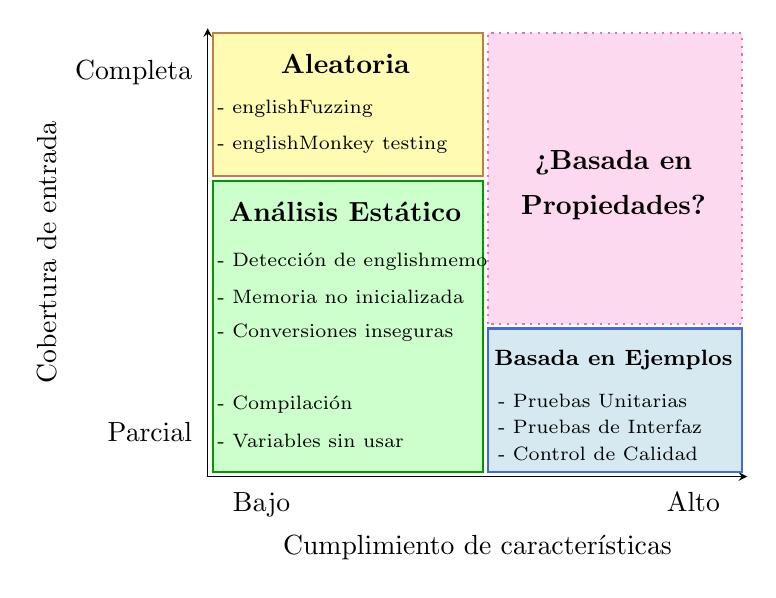
\begin{tikzpicture}
      axis line style={
         ->,
      },
      \begin{axis}[
         axis lines=left,
         xmin=0,
         xmax=1,
         xtick={0.1, 0.9},
         xticklabels={
            Bajo,
            Alto,
         },
         ymin=0,
         ymax=1,
         ytick={0.1, 0.9},
         yticklabels={
            Parcial,
            Completa,
         },
         tick style={draw=none},
         xlabel=Cumplimiento de características,
         ylabel=Cobertura de entrada
      ]
     
      \filldraw [
         fill=green!20!white,
         draw=green!60!black,
         thick,  
      ] (0.01,0.01) rectangle (0.51,0.66);

      \node[] at (axis cs: 0.255, 0.59) {\bfseries Análisis Estático};
      \node[anchor=west] at (axis cs: 0, 0.48) {\scriptsize- Detección de \fe{memory leak}};
      \node[anchor=west] at (axis cs: 0, 0.40) {\scriptsize- Memoria no inicializada};
      \node[anchor=west] at (axis cs: 0, 0.32) {\scriptsize- Conversiones inseguras};
      
      \node[anchor=west] at (axis cs: 0, 0.16) {\scriptsize- Compilación};
      \node[anchor=west] at (axis cs: 0, 0.08) {\scriptsize- Variables sin usar};

      \filldraw [
         fill=yellow!30!white,
         draw=brown,
         thick,  
      ] (0.01,0.67) rectangle (0.51,0.99);
      
      \node[] at (axis cs: 0.255, 0.92) {\bfseries Aleatoria};
      \node[anchor=west] at (axis cs: 0, 0.82) {\scriptsize- \fe{Fuzzing}};
      \node[anchor=west] at (axis cs: 0, 0.74) {\scriptsize- \fe{Monkey testing}};

      \filldraw [
         fill=lightblue!28!white,
         draw=lightblue!60!blue,
         thick,  
      ] (0.52,0.01) rectangle (0.99,0.33);
      
      \node[] at (axis cs: 0.752, 0.26) {\footnotesize\bfseries Basada en Ejemplos};
      \node[anchor=west] at (axis cs: 0.52, 0.17) {\scriptsize- Pruebas Unitarias};
      \node[anchor=west] at (axis cs: 0.52, 0.11) {\scriptsize- Pruebas de Interfaz};
      \node[anchor=west] at (axis cs: 0.52, 0.05) {\scriptsize- Control de Calidad};

      \filldraw [
         fill=magenta!15!white,
         draw=magenta!60!white,
         thick,
         dotted,
      ] (0.52,0.34) rectangle (0.99,0.99);

      \node[] at (axis cs: 0.752, 0.70) {\bfseries ¿Basada en};
      \node[] at (axis cs: 0.752, 0.60) {\bfseries Propiedades?};

      \end{axis}
   \end{tikzpicture}
   \begin{tabular}{@{}>{\small}m{.22\textwidth}|>{\small}l @{}}
      \multicolumn{1}{l|}{\small\textbf{Eje}}  &
      \multicolumn{1}{l}{\small\textbf{Significado}} \\[0.5ex]
      \hline
      Cumplimiento de \newline características & ¿Prueba realmente la funcionalidad que intento implementar? \\
      \hline
      Cobertura de entrada & ¿Cómo de bien cubro todos los posibles datos de entrada? \\
      \hline
   \end{tabular}
   
   \caption[Técnicas de pruebas automatizadas disponibles]{Técnicas de pruebas automatizadas disponibles (\emph{Fuente: }\cite{property-based-testing-article})
   \label{figura:property-based-testing}}
\end{figure}

La técnica usada para diseñarlas tiene como mayor exponente la librería \textbf{\fe{QuickCheck}} del lenguaje de programación \textbf{Haskell}, y consiste en \textbf{cambiar el enfoque} a la hora de crear pruebas unitarias. En lugar de buscar uno o varios ejemplos que abarquen los diferentes casos de uso de la funcionalidad a probar, \textbf{se indica} al propio \textbf{código} cómo puede \textbf{crear sus propios ejemplos} en base a una serie de \textbf{precondiciones} que todos ellos deben cumplir. Del mismo modo, el objetivo también cambia: cada prueba define una \textbf{propiedad} que la función debe cumplir. Estas propiedades tienen raíces matemáticas (producto de la naturaleza funcional\footnote{\url{https://es.wikipedia.org/wiki/Programaci\%C3\%B3n_funcional}} de Haskell), y suelen tener una estructura como la siguiente:

\begin{alltt}
   \newcommand{\vars}{(x, y, \dots)}

   para todo \vars
   
   donde la precondición \vars se cumple
   
   la propiedad \vars es verdadera
\end{alltt}

\subsubsection{Ejemplo práctico}

El siguiente ejemplo ha sido extraído de las pruebas unitarias de ``Al Loro''. La librería utilizada para implementar esta técnica se llama ``\emph{fast-check}'', y está disponible para JavaScript y TypeScript a través de la plataforma \emph{NPM}\footnote{\url{https://www.npmjs.com/package/fast-check}}.

\begin{lstlisting}[style=Typescript-no-dots,{deletekeywords=[3]{string}},{morekeywords=[5]{test, assert, asyncProperty, string, map, testSaveResponseForRepeatingInterceptor, expect, toEqual}},{morekeywords=[6]{SsmlOutputSpeech}},{keywordstyle=[5]\color{blue}},{keywordstyle=[6]\color{orange}}]
   // Repeat.test.ts
   import fc from 'fast-check';
   // ...
   test('works with ssml', async () => {
    await fc.assert(
      fc.asyncProperty(
        // Crea cadenas de texto rodeadas por la etiqueta "ssml"
        fc.string().map((str) => `<ssml>${str}</ssml>`),
        async (ssmlOutput) => {
          // Crea un objeto de tipo SSML con el texto generado
          const ssmlOutputSpeech: ui.SsmlOutputSpeech = {
            type: 'SSML',
            ssml: ssmlOutput,
          };
          // Prueba la función de repetición con el objeto
          // y obtiene el resultado
          const lastResponse = await testSaveResponseForRepeatingInterceptor(
            ssmlOutputSpeech
          );
          
          // Comprueba que la respuesta guardada coincide con el ejemplo
          expect(lastResponse).toEqual(ssmlOutput);
        }
      )
    );
  });
\end{lstlisting}

Este ejemplo está basado en la funcionalidad de repetición. Esta consiste en que cada respuesta que devuelve Alexa es guardada para que si el usuario dice: ``Repite'', Alexa repita el mismo mensaje.

Cuando Alexa manda una respuesta hablada, puede hacerlo con dos tipos de objetos: SSML (\fe{SsmlOutputSpeech}) o texto plano (\fe{PlainTextOutputSpeech}). Esta prueba se asegura de que la función es capaz de manejar objetos del primer tipo.

\section{Análisis estático} % Sonarqube
\label{seccion:analisis-estatico}

El \textbf{análisis estático} es una técnica basada en aplicar una serie de \textbf{reglas} al \textbf{código fuente} de una aplicación para identificar ciertos rasgos, normalmente asociados a la \textbf{calidad} y \textbf{seguridad} de dicho código.

La herramienta utilizada para ejecutar este tipo de análisis es \textbf{\fe{Sonarqube}}\footnote{\url{https://www.sonarqube.org/}}, una plataforma de código abierto (\fe{open-source}) especializada en aplicar análisis estático para detectar posibles defectos en tres principales áreas:

\begin{itemize}
   \item \textbf{Fiabilidad}: Este ámbito está compuesto únicamente de \textbf{\fe{bugs}}: segmentos de código considerados <<defectuosos>> al ser susceptibles de provocar errores o situaciones inesperadas.
   \item \textbf{Seguridad}
      \begin{itemize}
         \item \textbf{Vulnerabilidades}: Se tratan de comportamientos conocidos por suponer un riesgo para la seguridad del software, y normalmente requieren acción inmediata por parte del desarrollador.
         
         Ejemplos de esto son el uso de sistemas de cifrado considerados inseguros, o la implementación de código susceptible de ser manipulado por agentes externos (como utilizar datos proporcionados por el usuario para realizar consultas a una base de datos).
         \item \textbf{\fe{Hotspots}}: Este término, cuya traducción literal sería <<puntos calientes>>, simboliza aquel código que requiere una revisión exhaustiva por parte del desarrollador para determinar si supone un riesgo de seguridad. Aunque en algunos contextos podría no serlo, su uso ha sido un origen común de vulnerabilidades conocidas.
      \end{itemize}
   \item \textbf{Mantenibilidad}
      \begin{itemize}
         \item \textbf{\fe{Code Smells}}: Esta expresión hace referencia a aquellos fragmentos de código que <<huelen mal>>; es decir, que tienden a incurrir en malas prácticas, y por tanto son más propensos a errores y problemas de mantenibilidad tales como la falta de legibilidad.
         \item \textbf{Deuda técnica}: Es el tiempo estimado que le va a costar al desarrollador arreglar los problemas de mantenibilidad (principalmente los \fe{code smells}).
         
         Cuanto mayor sea este valor, menor será la productividad en el proceso de desarrollo, ya que la cantidad de tiempo empleada en solventar problemas se podría haber destinado a implementar nuevas funcionalidades.
      \end{itemize}
\end{itemize}

Además, tiene dos funcionalidades que Sonarqube no considera parte de la clasificación anterior:

\begin{itemize}
   \item \textbf{Detección de código duplicado}: Muestra un porcentaje de líneas duplicadas. Por defecto, considera la prueba de calidad fallida si este valor supera el tres por ciento.
   \item \textbf{Cobertura de código}: Esta funcionalidad requiere una integración con la librería de pruebas unitarias~(\ref{seccion:sonarqube-integracion-pruebas}), y muestra un informe de la cobertura de código por las pruebas existentes, indicando tanto un porcentaje general como una vista más detallada de cada fragmento de código.
\end{itemize}

\subsection{Descripción de la herramienta}% sonarqube-scanner, docker

El sistema que conforma \textbf{\fe{Sonarqube}} está compuesto por tres componentes (figura \ref{figura:sonarqube-system-arch}):

\begin{itemize}
   \item \textbf{Cliente}
      \begin{itemize}
         \item \textbf{Escáner}: Herramienta que analiza el código fuente y genera un informe con los resultados, el cual es enviado a través de HTTP al servidor principal.
      \end{itemize}
   \item \textbf{Servidor}
      \begin{itemize}
         \item \textbf{Servidor principal}: Es el encargado de procesar los resultados del informe, almacenarlos en la base de datos, y proporcionar al usuario con una interfaz y un sistema de búsqueda.
         \item \textbf{Base de datos}:
            Servidor externo\footnote{En la versión 8.9, Sonarqube admite los siguientes motores de base de datos: PostgreSQL, Microsoft SQL Server y Oracle.} donde se almacenan:
            \begin{itemize}
               \item Las métricas y problemas generados por el escáner.
               \item La configuración del servidor de Sonarqube.
            \end{itemize}
      \end{itemize}
\end{itemize}

\begin{figure}[ht]
   \centering
   \includegraphics[width=\textwidth]{SQ-instance-components.png}
   \caption[Arquitectura del sistema de Sonarqube]{Arquitectura del sistema de Sonarqube (\emph{Fuente: }\cite{sonarqube-doc})
   \label{figura:sonarqube-system-arch}}
\end{figure}

\subsection{Instalación y configuración}

\subsubsection{Servidor}% docker

Para instalar el servidor de \textbf{\fe{Sonarqube}}, existe una guía en la documentación oficial~\cite{sonarqube-doc}, la cual servirá de referencia en la siguiente descripción del proceso.

Aunque el servidor se puede instalar de forma manual, el método que se va a discutir en esta sección es aquel que implica utilizar la plataforma \textbf{\emph{Docker}}\footnote{\url{https://www.docker.com/}} (concretamente la herramienta \textbf{\emph{Docker Compose}}\footnote{\url{https://docs.docker.com/compose/}}), ya que facilita mucho el proceso de instalación y mantenimiento.

En el caso de ``Al Loro'', se decidió instalar \textbf{localmente}, en lugar de utilizar un servidor dedicado. Esto se debe a que, aunque el procedimiento habitual es el último, se trata de un proceso más costoso, y cuya ventaja es solamente notable en proyectos con un ciclo de vida más largo y/o con un mayor número de desarrolladores.

Para instalarlo mediante \emph{Docker Compose}, es necesario crear un archivo llamado ``\textbf{\emph{docker-compose.yml}}'' con la configuración de los servicios que conforman el entorno del servidor (sonarqube + base de datos). Por suerte, en la documentación oficial se incluye una versión de ejemplo completamente funcional:

\begin{lstlisting}[language=YAML]
   # docker-compose.yml

   version: "3"

   services:
     sonarqube:
       image: sonarqube:lts-community
       depends_on:
         - db
       environment:
         SONAR_JDBC_URL: jdbc:postgresql://db:5432/sonar
         SONAR_JDBC_USERNAME: sonar
         SONAR_JDBC_PASSWORD: sonar
       volumes:
         - sonarqube_data:/opt/sonarqube/data
         - sonarqube_extensions:/opt/sonarqube/extensions
         - sonarqube_logs:/opt/sonarqube/logs
         - sonarqube_temp:/opt/sonarqube/temp
       ports:
         - "9000:9000"
     db:
       image: postgres:12
       environment:
         POSTGRES_USER: sonar
         POSTGRES_PASSWORD: sonar
       volumes:
         - postgresql:/var/lib/postgresql
         - postgresql_data:/var/lib/postgresql/data
   
   volumes:
     sonarqube_data:
     sonarqube_extensions:
     sonarqube_logs:
     sonarqube_temp:
     postgresql:
     postgresql_data:   
\end{lstlisting}

Con este archivo y \emph{Docker Compose} instalado, es tan sencillo como llamar al comando ``\textbf{\emph{docker-compose up}}'' desde un terminal en la carpeta donde se encuentra el archivo. Este comando \textbf{instala} Sonarqube si no lo está y \textbf{lo inicia}.

La primera vez que se inicia, pedirá \textbf{usuario y contraseña}. Uno debe poner usuario ``\textbf{admin}'' y contraseña ``\textbf{admin}''. Una vez iniciada sesión, pedirá cambiar la contraseña. Deberás recordarla cada vez que inicies Sonarqube.

Para \textbf{parar el servidor} de Sonarqube, sólo hay que ejecutar el comando  ``\textbf{\emph{docker-compose down}}'' del mismo modo que se llamó al de inicio.

Para \textbf{desinstalarlo} completamente, se puede utilizar el comando ``\textbf{\emph{docker-compose down -v -~-rmi 'all'}}''\footnote{Ten en cuenta que el comando anterior eliminará tanto la imagen de Sonarqube como la de la base de datos, lo cual podría dar problemas en otros proyectos con Docker. Para evitar esto, elimina el parámetro <<\emph{-~- rmi 'all'}>> del comando, y desinstala la imagen de Sonarqube manualmente.} en su lugar, aunque es mejor \textbf{consultar la documentación}\footnote{\url{https://docs.docker.com/compose/reference/down/}} \textbf{antes} de ejecutarlo. 

Este sería el proceso habitual de instalación del servidor. Sin embargo, existe un pequeño \textbf{problema con los sistemas Linux}: existe un parámetro llamado ``\textbf{\emph{vm.max\_map\_count}}'' que debe valer como mínimo ``\textbf{\emph{524288}}'' para que Sonarqube funcione correctamente. Si no, lanza un error al iniciarse y no deja continuar.

Esto se puede arreglar \textbf{modificando este valor} de dos posibles formas (ambas requieren permisos de administrador):
\begin{itemize}
   \item \textbf{Temporalmente}: Mediante el comando ``\emph{sysctl -w vm.max\_map\_count=524288}'' se puede aplicar el cambio sólo para la sesión actual.
   \item \textbf{Permanentemente}: Se puede modificar el archivo de configuración ``\emph{/etc/sysctl.conf}'' o crear uno en ``\emph{/etc/sysctl.d/99-sonarqube.conf}'' para que utilicen este valor.
\end{itemize}

En el caso de una instalación \textbf{local}, lo más razonable es una opción \textbf{temporal}; ya que el dispositivo donde se instala tendrá más usos aparte de Sonarqube, y es probablemente mejor utilizar los valores por defecto en el resto de ocasiones.

En cambio, en una instalación en un \textbf{servidor dedicado} tendría más sentido la opción \textbf{permanente}, ya que ocurriría lo contrario que en la situación anterior.

Para facilitar el proceso de llamar a un comando más cada vez que se vaya a iniciar el servidor (para la solución temporal), se diseñó este \emph{script}:

\begin{lstlisting}[language=sh]
   # up.sh

   # Indica el programa con el que se debe ejecutar este script
   # (esta debe ser la primera línea del script)
   #!/bin/sh

   # Versiones 8.4 en adelante
   sonarqube_vm_max_map_count=524288
   # Versiones 8.3 o anteriores
   #sonarqube_vm_max_map_count=262144

   # Obtén el valor actual del parámetro
   current_vm_max_map_count="$(sysctl vm.max_map_count --values)"
  
   # Si el valor actual es menor al valor mínimo que requiere Sonarqube,
   # cámbialo por dicho mínimo
   [ $current_vm_max_map_count -lt $sonarqube_vm_max_map_count ] && sudo sysctl -w vm.max_map_count=$sonarqube_vm_max_map_count
   
   # Si el usuario actual es un miembro del grupo 'docker', no hacen falta permisos de administrador (obtenidos mediante el comando 'sudo')
   if id -Gn | grep -q '\bdocker\b'
   then
     docker-compose up -d
   else
     sudo docker-compose up -d
   fi    
\end{lstlisting}

\subsubsection{Cliente}% sonarqube-scanner

Para instalar el escáner de Sonarqube (llamado \textbf{\emph{SonarScanner}}) de forma local con soporte para JavaScript/TypeScript, es necesario instalar una herramienta de \textbf{CLI}. Esta se encuentra disponible en forma de archivos \textbf{binarios} para Linux, Windows o Mac (64 bits), como una \textbf{imagen Docker}, o como un \textbf{binario especial} que requiere tener pre-instalada la \textbf{JVM} (Java Virtual Machine).

Sin embargo, existe una librería en la plataforma \textbf{NPM} llamada ``\textbf{\emph{sonarqube-scanner}}'' (aunque no parece ser oficial) que encapsula el proceso de instalación y ejecución del escáner para poder hacerlo todo dentro del entorno de JavaScript. Se crea un archivo de este lenguaje llamando a la librería con la configuración adecuada, y así se puede ejecutar el escáner ejecutando el comando ``\textbf{\emph{node analyse.js}}'' (o con el nombre de archivo que uno quiera):

% En realidad es JavaScript, pero uso la language definition de TypeScript por conveniencia
\begin{lstlisting}[{morekeywords=[5]{require, scanner}},{keywordstyle=[5]\color{blue}}]
   // analyse.js

   const fs = require('fs');
   const scanner = require('sonarqube-scanner');
  
   // Obtiene el token de un archivo
   // (para evitar ponerlo en el propio código
   //  y así poder incluir este archivo en el sistema de control de versiones)
   const token = fs.readFileSync('./sonarqube/token.txt', 'utf-8').trim();
   
   scanner(
     {
       token: token,
       options: {
         'sonar.login': token,
         'sonar.projectName': 'Feed the Parrot',
         'sonar.sources': 'src/',
         'sonar.tests': 'tests/',
         'sonar.javascript.lcov.reportPaths': 'sonarqube/coverage/lcov.info',
         'sonar.testExecutionReportPaths': 'sonarqube/test-report.xml',
       },
     },
     () => process.exit()
   );
\end{lstlisting}

\subsection{Integración con las pruebas unitarias} % jest-sonar-reporter
\label{seccion:sonarqube-integracion-pruebas}

Para poder mostrar datos relacionados con la cobertura de las pruebas unitarias en el informe de Sonarqube, es necesaria una integración con la librería que las ejecuta.

En este caso, para integrar \textbf{\emph{jest}} con Sonarqube, se utiliza una librería llamada \textbf{\emph{jest-sonar-reporter}}. Esta es mencionada en la documentación de Sonarqube, y permite procesar los resultados del análisis de \emph{jest} en un formato que el escáner de Sonarqube comprenda.

Para ello, una vez instalada la librería de integración, es necesario \textbf{configurar} \emph{jest} para que haga uso de ella. Esto se puede lograr creando un archivo de configuración llamado ``\textbf{\emph{jest.config.js}}'' en la carpeta raíz del proyecto:

\begin{lstlisting}[style=Typescript-no-dots,{morekeywords=[5]{require}},{keywordstyle=[5]\color{blue}}]
   // jest.config.js

   const { defaults } = require('jest-config');
   module.exports = {
     preset: 'ts-jest',
     testEnvironment: 'node',
     testResultsProcessor: 'jest-sonar-reporter',
     coverageDirectory: 'sonarqube/coverage',
     coveragePathIgnorePatterns: [
       ...defaults.coveragePathIgnorePatterns,
       '<rootDir>/tests/helpers/',
     ],
   };

\end{lstlisting}

De este modo, cada vez que se ejecute el comando ``\textbf{\emph{jest -~-coverage}}'' para analizar la cobertura de las pruebas, se creará un informe compatible con Sonarqube en la carpeta definida como ``\emph{coverageDirectory}''.

%\section{?? ???? ???? ? ?? ??}
%
%????? ????????????? ????????????? ????????????? ????????????? ?????????????

%%%%%%%%%%%%%%%%%%%%%%%%%%%%%%%%%%%%%%%%%%%%%%%%%%%%%%%%%%%%%%%%%%%%%%%%%%%%%%%
%                                 CONCLUSIONES                                 %
%%%%%%%%%%%%%%%%%%%%%%%%%%%%%%%%%%%%%%%%%%%%%%%%%%%%%%%%%%%%%%%%%%%%%%%%%%%%%%%

\chapter{Conclusiones}
\label{capitulo:conclusiones}

\section{Objetivos cumplidos}

A lo largo del contenido de este trabajo, se ha hecho un \textbf{repaso} del \textbf{proceso de desarrollo} de la skill <<Al Loro>>.

Para ello, se ha detallado el proceso de integración de una skill con servicios de \textbf{base de datos} tanto incluidos por Amazon (\emph{DynamoDB}) como externos (\emph{Firebase}).

Además, se ha implementado una \textbf{app} con \emph{Flutter}, se ha seguido su proceso de implantación en Android, y se ha creado un método de \textbf{comunicación entre la skill y la app} a través de una \emph{API} (para el servicio de autenticación) y de una base de datos en \emph{Firebase}.

Por otro lado, se ha documentado el funcionamiento de una \textbf{interfaz} guiada por voz, presentando \textbf{ejemplos} en base al desarrollo de una \textbf{skill real} (<<Al Loro>>).

También se han comentado los \textbf{servicios de \emph{AWS}} que se ofrecen desde Alexa, y se ha profundizado en la \textbf{lógica de la skill} enseñando el modo de uso del \textbf{\emph{ASK SDK}}, el cual presenta grandes similitudes con librerías y herramientas típicas del \textbf{desarrollo \fe{backend}}.

\section{Relación del trabajo desarrollado con los estudios cursados}

Varios conceptos aprendidos en las asignaturas \textbf{AVD} (Análisis, validación y depuración de software) y \textbf{MES} (Mantenimiento y evolución de software) han sido utilizados para implementar las \hyperref[capitulo:pruebas]{\textbf{pruebas}} unitarias:

\begin{itemize}
   \item \nameref{seccion:mocks}
   \item \nameref{seccion:property-based-testing}
   \item \nameref{seccion:analisis-estatico} (\emph{Sonarqube})
\end{itemize}

Asimismo, los conocimientos acerca de la gestión de proyectos de asignaturas como \textbf{PSW} (Proceso de software) o \textbf{PIN} (Proyecto de ingeniería de software) han sido útiles para \hyperref[seccion:gestion-proyecto]{administrar un tablero kanban en \emph{Trello}}. Aunque la mejora habría sido más notable en un trabajo en grupo, ideas como la clasificación de tareas según su estado o el etiquetado en función de su prioridad y dificultad ayudaron a organizar mejor el proyecto y aumentar la productividad.

\section{Aprendizaje, retos y dificultades}

El principal desafío que ha supuesto el desarrollo de la skill ha sido la adaptación al entorno de implementar y mantener un software en producción, ya que surgen problemas que no se suelen tener en cuenta en un proyecto de carrera.

Por ejemplo, una decisión importante es la de elegir una plataforma donde alojar un servicio web. Para ello, no sólo hay que tener en cuenta el precio, sino también cuestiones de seguridad, funcionalidad; o, en proyectos más grandes, la capacidad de escalar (es decir, de poder lidiar con una carga de trabajo mayor, normalmente por tener un mayor número de usuarios).

Cuando se elige una plataforma menos adecuada para el tipo de servicio que uno busca ofrecer, pueden surgir una serie de problemas nuevos. Este fue el caso del servicio de autenticación, donde al elegir \emph{Firebase Functions}, la \emph{API} recibió un ataque de peticiones en masa (probablemente con el objetivo de obtener acceso a cuentas de usuario). \hyperref[seccion:migracion-auth]{Migrando el servicio} a \emph{AWS} se solucionó el problema, pero resultó en un trabajo extra que se podría haber evitado.

Otra lección obtenida gracias a este trabajo ha sido la de saber cuándo vale la pena invertir tiempo en arreglar un problema y cuándo no (especialmente cuando no tiene fácil solución).

Esto fue resultado de una limitación de Alexa: tiene un número \hyperref[seccion:limite-caracteres]{máximo de caracteres en una respuesta}, y cuando la noticia era demasiado larga, daba un error que el usuario no podía entender y se cerraba. En la documentación indica un número exacto de caracteres, pero en la práctica esto no se cumplía. Por tanto, la idea inicial fue probar distintas longitudes para tratar de dar con un número mágico a partir del cual fallara, y así poder comprobar con relativa facilidad esta condición; si se daba, se podría avisar al usuario.

Sin embargo, esta tarea resultó ser demasiado compleja. En cuanto se dio con un número lo suficientemente bueno como para que la probabilidad de error fuese bastante baja, se consideró que no merecía la pena continuar buscando una mejor solución.

Finalmente, el mayor aprendizaje ha sido el de aprender una nueva tecnología desde cero, documentar el proceso y tratar de crear un puente entre los procesos existentes y estas nuevas prácticas. Espero que el contenido de este trabajo pueda ayudar a desarrolladores que busquen iniciarse en este nuevo campo, y que logren implementar aquello que se propongan.


%%%%%%%%%%%%%%%%%%%%%%%%%%%%%%%%%%%%%%%%%%%%%%%%%%%%%%%%%%%%%%%%%%%%%%%%%%%%%%%
%                                BIBLIOGRAFÍA                                 %
%%%%%%%%%%%%%%%%%%%%%%%%%%%%%%%%%%%%%%%%%%%%%%%%%%%%%%%%%%%%%%%%%%%%%%%%%%%%%%%

\begin{thebibliography}{10}

\bibitem{google-assistant-docs}
   Documentación disponible sobre el asistente de Google.\\
   \newblock \url{https://developers.google.com/assistant/docs}

\bibitem{alexa-skills-docs}
   Documentación disponible sobre las Alexa skills.\\
   \newblock \url{https://developer.amazon.com/es-ES/docs/alexa/ask-overviews/what-is-the-alexa-skills-kit.html}

\bibitem{siri-docs}
   Documentación disponible sobre el kit de desarrollo para Siri (SiriKit).\\
   \newblock \url{https://developer.apple.com/documentation/sirikit}

\bibitem{voice-search-study}
   Estudios sobre los diferentes asistentes de voz y sus sistemas de búsqueda.\\
   \newblock \url{https://www.semrush.com/blog/voice-search-local-seo/}
   
\bibitem{voice-assistant-market-share}
   Informe realizado por \emph{voicebot.ai} en 2020 sobre la cuota relativa de mercado de los asistentes de voz en \fe{smartphones} de Estados Unidos.\\
   \newblock \url{https://voicebot.ai/2020/11/05/voice-assistant-use-on-smartphones-rise-siri-maintains-top-spot-for-total-users-in-the-u-s/}

\bibitem{alexa-hosted-skill}
   Documentación acerca de las Alexa-hosted skills.\\
   \newblock \url{https://developer.amazon.com/es-ES/docs/alexa/hosted-skills/build-a-skill-end-to-end-using-an-alexa-hosted-skill.html}

\bibitem{ask-cli-migration-guide}
   Alexa Developer - Guía de migración del ASK CLI de la versión 1 a la 2.\\
   \newblock \url{https://developer.amazon.com/es-ES/docs/alexa/smapi/ask-cli-v1-to-v2-migration-guide.html}

\bibitem{alexa-hooks-related-blogpost}
   Artículo en el blog de Alexa donde se comenta la existencia de la funcionalidad ``\fe{hook scripts}'' a partir de la versión 1.5 del ASK CLI.\\
   \newblock \url{https://developer.amazon.com/es/blogs/alexa/post/89782c5d-6d3f-488c-843b-751656afc3c8/python-skill-development-now-supported-in-the-ask-cli-and-ask-toolkit-for-visual-studio-code}

\bibitem{git-hooks-doc}
   Documentación acerca de la funcionalidad ``\fe{hooks}'' en la herramienta de control de versiones \emph{Git}.
   \newblock
      \begin{itemize}
         \item En inglés: \url{https://git-scm.com/book/en/v2/Customizing-Git-Git-Hooks}
         \item En español: \url{https://git-scm.com/book/es/v2/Personalizaci%C3%B3n-de-Git-Puntos-de-enganche-en-Git}
      \end{itemize}

\bibitem{flash-briefing-skills-doc}
   Documentación sobre las \fe{flash briefing} skills (skills que siguen el modelo de noticias)\\
   \newblock \url{https://developer.amazon.com/es-ES/docs/alexa/flashbriefing/understand-the-flash-briefing-skill-api.html} 

\bibitem{flash-briefing-skill-policy-guidelines}
   Directrices relacionadas con la política de Alexa.\\
   \newblock \url{https://developer.amazon.com/es-ES/docs/alexa/flashbriefing/flash-briefing-skill-certification-checklist.html#policyGuidelines}

\bibitem{flash-briefing-skill-certification-process}
   Lista de requisitos para completar con éxito el proceso de certificación de una skill de noticias.\\
   \newblock \url{https://developer.amazon.com/es-ES/docs/alexa/flashbriefing/flash-briefing-skill-certification-checklist.html}

\bibitem{flash-briefing-skill-feed-format-details}
   Tabla con los elementos necesarios para una feed en una skill de noticias, y su formato adecuado.\\
   \newblock \url{https://developer.amazon.com/es-ES/docs/alexa/flashbriefing/flash-briefing-skill-api-feed-reference.html#details}

\bibitem{flash-briefing-skill-text-content-requirements}
   Requisitos del contenido textual de una feed en una skill de noticias.\\
   \newblock \url{https://developer.amazon.com/es-ES/docs/alexa/flashbriefing/flash-briefing-skill-api-feed-reference.html#text-content-requirements}

\bibitem{apl-doc}
   Documentación acerca del \emph{APL} (\fe{Alexa Presentation Language}).\\
   \newblock \url{https://developer.amazon.com/es-ES/docs/alexa/alexa-presentation-language/understand-apl.html}

\bibitem{property-based-testing-article}
   Artículo: \fe{Introduction to Property Based Testing} (\fe{Medium}).\\
   \newblock \url{https://medium.com/criteo-engineering/introduction-to-property-based-testing-f5236229d237}

\bibitem{sonarqube-doc}
   Sonarqube - Documentación oficial (versión 8.9 LTS).\\
   \newblock \url{https://docs.sonarqube.org/8.9/}


% spell-checker: disable
%%%%%%%%%%%%%%%%%%%%%%%%%%%%%%%%%%%%%%%%%%%%%%%%%%%%%%%%%%%%%%%%%%%%%%%%%%%%%%%
% MODEL D'ARTICLE                                                             %
%%%%%%%%%%%%%%%%%%%%%%%%%%%%%%%%%%%%%%%%%%%%%%%%%%%%%%%%%%%%%%%%%%%%%%%%%%%%%%%
%\bibitem{light}
%   Jennifer~S. Light.
%   \newblock When computers were women.
%   \newblock \textit{Technology and Culture}, 40:3:455--483, juliol, 1999.

%%%%%%%%%%%%%%%%%%%%%%%%%%%%%%%%%%%%%%%%%%%%%%%%%%%%%%%%%%%%%%%%%%%%%%%%%%%%%%%
% MODEL DE LLIBRE                                                             %
%%%%%%%%%%%%%%%%%%%%%%%%%%%%%%%%%%%%%%%%%%%%%%%%%%%%%%%%%%%%%%%%%%%%%%%%%%%%%%%
%\bibitem{ifrah}
%   Georges Ifrah.
%   \newblock \textit{Historia universal de las cifras}.
%   \newblock Espasa Calpe, S.A., Madrid, sisena edició, 2008.

%%%%%%%%%%%%%%%%%%%%%%%%%%%%%%%%%%%%%%%%%%%%%%%%%%%%%%%%%%%%%%%%%%%%%%%%%%%%%%%
% MODEL D'URL                                                                 %
%%%%%%%%%%%%%%%%%%%%%%%%%%%%%%%%%%%%%%%%%%%%%%%%%%%%%%%%%%%%%%%%%%%%%%%%%%%%%%%
%\bibitem{WAR}
%   Comunicat de premsa del Departament de la Guerra, 
%   emés el 16 de febrer de 1946. 
%   \newblock Consultat a 
%   \url{http://americanhistory.si.edu/comphist/pr1.pdf}.

% spell-checker: enable
   
\end{thebibliography}
\cleardoublepage

%%%%%%%%%%%%%%%%%%%%%%%%%%%%%%%%%%%%%%%%%%%%%%%%%%%%%%%%%%%%%%%%%%%%%%%%%%%%%%%
%                           APÉNDICES  (Si los hay)                           %
%%%%%%%%%%%%%%%%%%%%%%%%%%%%%%%%%%%%%%%%%%%%%%%%%%%%%%%%%%%%%%%%%%%%%%%%%%%%%%%

\APPENDIX

%%%%%%%%%%%%%%%%%%%%%%%%%%%%%%%%%%%%%%%%%%%%%%%%%%%%%%%%%%%%%%%%%%%%%%%%%%%%%%%
%                         LA CONFIGURACIÓN DEL SISTEMA                        %
%%%%%%%%%%%%%%%%%%%%%%%%%%%%%%%%%%%%%%%%%%%%%%%%%%%%%%%%%%%%%%%%%%%%%%%%%%%%%%%

\chapter{Manual de usuario (Skill)}

\section{Instalación}

\subsection{Como usuario}

Alexa instala automáticamente las skills cuando el usuario pide abrirlas por primera vez. Por tanto, instalar esta skill es tan sencillo como decirle a Alexa: <<Abre Al Loro>>\footnote{Esto solo funcionaría si la skill hubiera sido aprobada tras un proceso de certificación y se encontrara en producción. En el caso de <<Al Loro>> no lo está, pues la certificación es compleja, requiere comunicación con el equipo de Amazon, y se consideró que no merecía la pena ya que no hay intención de mantenerla más allá de la duración de este trabajo.} (figura \ref{figura:comando-abrir-skill}).

\begin{figure}[ht]
   \centering
   \includegraphics[width=\textwidth]{abrir.png}
   \caption{Comando: Abrir la skill}
   \label{figura:comando-abrir-skill}
\end{figure}

\subsection{Como desarrollador}

Para activar la skill como desarrollador, se debe utilizar la \textbf{app de Alexa}. Los pasos son:

\includegraphics[width=0.4\textwidth]{activate-skill-1.jpg}
\includegraphics[width=0.4\textwidth]{activate-skill-2.jpg}

\begin{enumerate}
   \item Pulsar el botón <<\textbf{Más}>>, situado en la esquina inferior derecha.
   \item Acceder a la sección <<\textbf{Skills y juegos}>>.
  
   \raggedbottom

   \includegraphics[width=0.4\textwidth]{activate-skill-3.jpg}
   \includegraphics[width=0.4\textwidth]{activate-skill-4.jpg}

   \item En la barra superior, pulsar <<\textbf{Mis Skills}>>.
   \item Pulsar sobre el cuadro <<\textbf{Desarrollador}>>.
   
   \includegraphics[width=0.4\textwidth]{activate-skill-5.jpg}
   \includegraphics[width=0.4\textwidth]{activate-skill-6.jpg}

   \item Si todo va bien, aparecerá la skill en una lista. Pulsar sobre ella.
   \item Pulsar el botón <<\textbf{Permitir su uso}>>.
\end{enumerate}

\subsection{Como beta tester}

Existe una opción de \fe{beta testing}\footnote{\url{https://developer.amazon.com/en-US/docs/alexa/custom-skills/skills-beta-testing-for-alexa-skills.html}} para el desarrollador, donde puede invitar a un máximo de 500 testers durante un periodo de hasta 90 días para que prueben la skill.

En este caso, es el desarrollador el que debe incluir a los testers añadiendo su dirección de correo electrónico a una lista. Una vez habilitado el beta test, se mandarán automáticamente correos a estas direcciones con un enlace a través del cual pueden instalar la skill tras iniciar sesión.

\section{Comandos disponibles}

\begin{itemize}
   \item \textbf{Lee una feed}: También se puede llamar como <<lee la feed \{\emph{nombre de la feed}\}>> para indicarla directamente (figura \ref{figura:comando-leer-feed}). Si no se indica, Alexa preguntará por su nombre (figura \ref{figura:comando-leer-feed-sin-nombre}).
   
   Para ver el árbol de decisión tras invocar este comando, se puede observar el diagrama de flujo para este caso de uso de la figura \ref{figura:diagrama-flujo}.

   También existen mensajes de error personalizados para cuando una feed es inválida (figura \ref{figura:error-feed-invalida}) o es demasiado larga (figura \ref{figura:error-feed-larga}).
   \item \textbf{Lista de feeds} (figura \ref{figura:comando-lista-feeds})
   \item \textbf{Iniciar sesión} (figura \ref{figura:comando-iniciar-sesion}): Genera un código de seis dígitos para iniciar sesión desde la app. Tiene un periodo de validez de diez minutos; pasado ese tiempo, se debe generar un nuevo código.
   \item \textbf{Ayuda}: Lee una descripción general de los comandos disponibles.
\end{itemize}

\begin{figure}[ht]
   \centering
   \includegraphics[width=.9\textwidth]{leer-feed-sin-nombre.png}
   \caption{Comando: Leer una feed (sin indicar el nombre)}
   \label{figura:comando-leer-feed-sin-nombre}
\end{figure}

\begin{figure}[ht]
   \centering
   \includegraphics[width=.9\textwidth]{lista-feeds.png}
   \caption{Comando: Lista de feeds}
   \label{figura:comando-lista-feeds}
\end{figure}

\begin{figure}[ht]
   \centering
   \includegraphics[width=.9\textwidth]{iniciar-sesion.png}
   \caption{Comando: Iniciar sesión}
   \label{figura:comando-iniciar-sesion}
\end{figure}

\begin{figure}[ht]
   \centering
   \includegraphics[width=.9\textwidth]{feed-invalida.png}
   \caption{Error: Feed inválida}
   \label{figura:error-feed-invalida}
\end{figure}

\begin{figure}[!htb]
   \centering
   \includegraphics[width=.9\textwidth]{feed-demasiado-larga.png}
   \caption{Error: Feed demasiado larga}
   \label{figura:error-feed-larga}
\end{figure}

\begin{figure}[ht]
   \centering
   \includegraphics[width=.602\textwidth]{leer-feed.png}
   \caption{Comando: Leer una feed}
   \label{figura:comando-leer-feed}
\end{figure}

\section{Lista completa de comandos}

En primer lugar, es importante mencionar que existen una serie de comandos que vienen predefinidos por Amazon. En estos casos, la lista completa no está disponible. Ejemplos son: <<cancelar>>, <<parar>>, <<sí>>, <<no>>, etc.

Los comandos predefinidos también pueden ser expandidos con mensajes personalizados que los activen. El ejemplo más claro en esta skill es el del comando <<ayuda>>.

A continuación se muestra la lista completa de comandos personalizados con todas las posibles formas de invocar cada uno:

\begin{itemize}
   \item \textbf{Leer una feed}:
   \begin{itemize}
      \item <<di las noticias de la feed \{feed\}>>
      \item <<di las noticias>>
      \item <<que diga las noticias de la feed \{feed\}>>
      \item <<que diga las noticias>>
      \item <<que me dé las noticias de la feed \{feed\}>>
      \item <<que me dé las noticias>>
      \item <<dame las noticias de la feed \{feed\}>>
      \item <<dame las noticias>>
      \item <<que me diga las noticias de la feed \{feed\}>>
      \item <<que me diga las noticias>>
      \item <<dime las noticias de la feed \{feed\}>>
      \item <<dime las noticias>>
      \item <<que me dé la feed \{feed\}>>
      \item <<dime qué hay en la feed \{feed\}>>
      \item <<dime qué hay>>
      \item <<que me diga qué hay en la feed \{feed\}>>
      \item <<que me diga qué hay>>
      \item <<que me lea la feed \{feed\}>>
      \item <<que me lea una feed>>
      \item <<que lea la feed \{feed\}>>
      \item <<que lea una feed>>
      \item <<qué hay en la feed \{feed\}>>
      \item <<dame la feed \{feed\}>>
      \item <<léeme la feed \{feed\}>>
      \item <<lee la feed \{feed\}>>
      \item <<léeme una feed>>
      \item <<lee una feed>>
   \end{itemize}
   \item \textbf{Leer una feed - Indicar nombre}:
   \begin{itemize}
      \item <<Se trata de la feed \{feed\}>>
      \item <<Se trata de \{feed\}>>
      \item <<Es \{feed\}>>
      \item <<Es la feed \{feed\}>>
      \item <<La feed se llama \{feed\}>>
      \item <<Se llama \{feed\}>>
      \item <<\{feed\}>>
   \end{itemize}
   \item \textbf{Lista de feeds}:
   \begin{itemize}
      \item <<que me diga qué feeds tiene disponibles>>
      \item <<que me diga qué feeds tiene>>
      \item <<que me diga qué feeds tengo>>
      \item <<que me diga qué feeds tengo disponibles>>
      \item <<que me diga la lista de feeds>>
      \item <<que me dé la lista de feeds>>
      \item <<lista de feeds>>
      \item <<lista>>
      \item <<dame la lista>>
      \item <<dime la lista>>
      \item <<dime la lista de feeds>>
      \item <<dame la lista de feeds>>
      \item <<qué feeds tienes disponibles>>
      \item <<qué feeds tienes>>
      \item <<qué feeds hay disponibles>>
      \item <<qué feeds hay>>
      \item <<qué feeds tengo disponibles>>
      \item <<qué feeds tengo>>
   \end{itemize}
   \item \textbf{Iniciar sesión}:
   \begin{itemize}
      \item <<login>>
      \item <<iniciar sesión>>
      \item <<código para iniciar sesión>>
      \item <<dame el código para iniciar sesión>>
   \end{itemize}
   \item \textbf{Ayuda} \emph{(Predefinido por Amazon)}:
   \begin{itemize}
      \item <<qué puedo hacer>>
      \item <<cómo puedo gestionar mis feeds>>
      \item <<cómo gestionar mis feeds>>
      \item <<cómo inicio sesión desde la app>>
      \item <<cómo iniciar sesión desde la app>>
   \end{itemize}
\end{itemize}

\chapter{Manual de usuario (App)}

La app está formada por las siguientes pantallas:

\begin{itemize}
   \item \textbf{Inicio sesión} (figura \ref{figura:app-iniciar-sesion}): En esta pantalla se debe introducir un código que la skill dictó previamente al invocar el comando <<iniciar sesión>>.
   \item \textbf{Gestión de feeds} (figura \ref{figura:app-gestion-feeds}): Muestra una lista de las feeds disponibles. Pueden seleccionarse con los recuadros de la izquierda para luego ser eliminadas con el botón de abajo, se pueden editar pulsando sobre el icono del lápiz, y se pueden crear nuevas pulsando sobre el botón <<Nueva>> (también situado abajo).
   
   Para cerrar sesión, se debe pulsar el botón situado en la esquina superior derecha.
   \item \textbf{Nueva / Editar feed}: Además de los campos básicos como el nombre, el idioma, o la URL (figura \ref{figura:app-editar-feed}), también tiene una serie de opciones para limitar el tamaño de la feed o para filtrarla por texto y/o categorías (figura \ref{figura:app-editar-feed-opciones}).
\end{itemize}

\begin{figure}[ht]
   \centering
   \includegraphics[width=.9\textwidth]{app-iniciar-sesion.png}
   \caption{App: Iniciar sesión}
   \label{figura:app-iniciar-sesion}
\end{figure}

\begin{figure}[ht]
   \centering
   \includegraphics[width=.9\textwidth]{app-gestion-feeds.png}
   \caption{App: Gestionar feeds}
   \label{figura:app-gestion-feeds}
\end{figure}

\begin{figure}[ht]
   \centering
   \includegraphics[width=.9\textwidth]{app-editar-feed.png}
   \caption{App: Nueva/Editar feed}
   \label{figura:app-editar-feed}
\end{figure}

\begin{figure}[ht]
   \centering
   \includegraphics[width=.74\textwidth]{app-editar-feed-opciones.jpg}
   \caption{App: Nueva/Editar feed - Opciones}
   \label{figura:app-editar-feed-opciones}
\end{figure}

%%%%%%%%%%%%%%%%%%%%%%%%%%%%%%%%%%%%%%%%%%%%%%%%%%%%%%%%%%%%%%%%%%%%%%%%%%%%%%%
%                               OTROS  APÉNDICES                              %
%%%%%%%%%%%%%%%%%%%%%%%%%%%%%%%%%%%%%%%%%%%%%%%%%%%%%%%%%%%%%%%%%%%%%%%%%%%%%%%

\chapter{Glosario}
\label{glosario}

\begin{description}
   \item [Feed:] \label{glosario:feed} Listado de artículos web con un formato estandarizado, normalmente utilizado en blogs o sitios de noticias para poder difundir sus contenidos fácilmente en otros servicios o páginas web. Estos suelen ser actualizados cada cierto tiempo.
   \item [ASK:] \label{glosario:ASK} (Acrónimo de ``\fe{Alexa Skills Kit}'') Conjunto de herramientas proporcionadas por Amazon para el desarrollo de skills en Alexa.
   \item [CLI:] \label{glosario:CLI} (Acrónimo de ``\fe{Command Line Interface}''): Programa desarrollado para ser utilizado mediante la línea de comandos.
\end{description}

%%%%%%%%%%%%%%%%%%%%%%%%%%%%%%%%%%%%%%%%%%%%%%%%%%%%%%%%%%%%%%%%%%%%%%%%%%%%%%%
%                              FIN DEL DOCUMENTO                              %
%%%%%%%%%%%%%%%%%%%%%%%%%%%%%%%%%%%%%%%%%%%%%%%%%%%%%%%%%%%%%%%%%%%%%%%%%%%%%%%

\end{document}
